
% ============================================================
% IST / Elsevier elsarticle format
% Compile on Overleaf (elsarticle.cls available by default)
% ===========================================================
\documentclass[preprint,number]{elsarticle}
% ===========================================================
% PACKAGES
% ============================================================
\usepackage[utf8]{inputenc}
\usepackage[T1]{fontenc}
\usepackage{lineno}
\modulolinenumbers[5]
\usepackage{amsmath,amssymb}
\usepackage{graphicx}
\usepackage{textcomp}
\usepackage{xcolor}
\usepackage{booktabs}
\usepackage{array}
\usepackage{multirow}
\usepackage{colortbl}
\usepackage{tabularx}
\usepackage{float}
\usepackage[section]{placeins} % keep each section's floats inside that section (no drift past the appendix)
\usepackage{longtable}
\usepackage{url}
\usepackage[hidelinks]{hyperref}
\usepackage{enumitem}
\usepackage{tikz}
\usepackage{pgfplots}
\pgfplotsset{compat=1.17}
\usetikzlibrary{
  shapes.geometric,
  shapes.multipart,
  arrows.meta,
  positioning,
  calc,
  fit,
  backgrounds,
  decorations.pathreplacing
}
\usepackage[most]{tcolorbox}
% ============================================================
% COLOR DEFINITIONS
% ============================================================
\definecolor{acmblue}{RGB}{0,51,102}
\definecolor{tableheader}{RGB}{220,230,242}
\definecolor{lightgray}{RGB}{245,245,245}
\definecolor{prismaID}{RGB}{41,98,255}
\definecolor{prismaScreen}{RGB}{124,58,237}
\definecolor{prismaElig}{RGB}{220,38,38}
\definecolor{prismaInc}{RGB}{5,150,105}
\definecolor{prismaBox}{RGB}{241,245,249}
\definecolor{prismaExcl}{RGB}{254,226,226}
\definecolor{prismaOther}{RGB}{255,247,237}
\definecolor{catA}{RGB}{31,119,180}
\definecolor{catB}{RGB}{255,127,14}
\definecolor{catC}{RGB}{44,160,44}
\definecolor{catD}{RGB}{214,39,40}
\definecolor{catE}{RGB}{148,103,189}
\definecolor{catF}{RGB}{140,86,75}
\definecolor{wlcolor}{RGB}{65,105,225}
\definecolor{glcolor}{RGB}{50,205,50}

\hypersetup{
    colorlinks=true,
    linkcolor=acmblue,
    citecolor=acmblue,
    urlcolor=acmblue
}

% Citations: academic sources of the review are ordinary references (\cite{ID}, keyed by corpus ID in
% references.bib). Gray literature sources keep their own identifier, GL1--GL75, keyed to the appendix table.
\biboptions{numbers,sort&compress}
\newcounter{study}
\renewcommand{\thestudy}{GL\arabic{study}}
\newcommand{\refG}[1]{\ref{s:#1}}
\setlength{\emergencystretch}{2em} % lets paragraphs with long citation lists break without overfull lines

% >>> FLOAT PLACEMENT TUNING >>>
% Let text share pages with figures/tables and avoid sparse float-only pages.
\setcounter{topnumber}{3}          % up to 3 floats at the top of a text page
\setcounter{bottomnumber}{2}       % up to 2 floats at the bottom
\setcounter{totalnumber}{4}        % up to 4 floats on a single text page
\renewcommand{\topfraction}{0.92}      % a text page may be up to 92% float at top
\renewcommand{\bottomfraction}{0.85}   % ... and up to 85% at bottom
\renewcommand{\textfraction}{0.07}     % require only 7% text on a mixed page
\renewcommand{\floatpagefraction}{0.80}% a float-only page must be >=80% full
\setcounter{dbltopnumber}{3}
\renewcommand{\dbltopfraction}{0.92}
\renewcommand{\dblfloatpagefraction}{0.80}
% <<< FLOAT PLACEMENT TUNING <<<

% Elsarticle journal metadata
\journal{Information and Software Technology}

% ============================================================
\begin{document}

\begin{frontmatter}

\title{Past, Present, and Future of Developer Productivity Measurement: A Multivocal Literature Review}

%\author[anon]{Anonymous Author\corref{cor1}}
\author[a]{Rafael Rampin Soratto\corref{cor1}}
\ead{pg56642@uem.br}
\author[d]{Getúlio Coimbra}
\author[b]{Jorge Melegati}
\author[c]{Igor Steinmacher}
\author[a]{Igor Wiese}
\cortext[cor1]{Corresponding author}
\address[a]{Graduate Program in Computer Science, State University of Maringá (UEM), Maringá, Paraná, Brazil}
\address[b]{INESC TEC, Faculty of Engineering, University of Porto, Porto, Portugal}
\address[c]{Northern Arizona University, Flagstaff, Arizona, USA}
\address[d]{Federal University of Technology -- Paraná (UTFPR), Campo Mourão, Paraná, Brazil}

% ============================================================
% ABSTRACT
% ============================================================
\begin{abstract}
\noindent\textit{\textbf{Context:}}
Since software development is a form of knowledge work, measuring developer productivity has long been challenging. Counting lines of code, commits, or story points does not give a full picture of what developers contribute, and measures of developer experience have been introduced to complement them.

\noindent\textit{\textbf{Objectives:}}
This study aims to understand how developer productivity measurement has changed since the COVID-19 pandemic and the emergence of generative AI, and whether proposed frameworks have been used to measure it.

\noindent\textit{\textbf{Method:}}
We conducted a multivocal literature review (MLR) covering the pre-pandemic (2016--2019), pandemic (2020--2022), and post-pandemic and AI (2023--2026) periods. Systematic database searches and a purposive gray literature search yielded 228 sources, 153 academic and 75 gray. We analyzed the metrics, frameworks, and tools used, and how remote work, AI assistants, and context affected them.

\noindent\textit{\textbf{Results:}}
DORA, SPACE, and DevEx were cited in both academic and gray literature, and their use as measurement instruments became more prevalent after 2022. Academic studies cite these frameworks more often than they use them. Gray sources use DORA to measure more often than academic studies (16.0\% vs. 5.9\%). This gap comes from vendor and maintainer sources (30.3\%), as independent gray sources (4.8\%) are close to academic studies. Studies of AI assistants tend to report output gains, while those that also measure quality or review effort report costs that offset part of them.

\noindent\textit{\textbf{Conclusion:}}
Across the decade, what changed is less which framework is used than what is measured alongside output. No single framework appears to cover all dimensions of developer productivity. Future studies, especially of AI-assisted work, could combine delivery, perception, and experience measures at the individual, team, and system levels. Validated DevEx instruments, longitudinal designs, and evidence on the team- and system-level effects of AI assistants are still needed.
\end{abstract}

\begin{keyword}
software developer productivity \sep DORA metrics \sep SPACE framework \sep developer experience \sep AI coding assistants \sep multivocal literature review
\end{keyword}

\end{frontmatter}

\linenumbers  % enabled for review submission (IST requires line numbers; comment out for a clean preprint layout)

% ============================================================
% 1. INTRODUCTION
% ============================================================
\section{Introduction}
\label{sec:introduction}

Software engineering has long measured what it can count. Lines of code and commits have served as proxies for evaluating product and process aspects such as defect prediction~\cite{basili1996validation, nagappan2005churn, zimmermann2007predicting}, change impact analysis~\cite{bohner1996impact, arnold1993impact}, technical debt~\cite{cunningham1992wycash, kruchten2012td, seaman2011td}, and the productivity of both software and developers~\cite{boehm1981economics, albrecht1983function, jones1986productivity}. Underlying this practice is an input-and-output model of development, in which greater output equates to higher productivity~\cite{kupiainen2015metrics}. Software development, however, is knowledge work: creative, collaborative, and difficult to quantify~\cite{P1259}. Human factors such as job enthusiasm and peer support have predicted self-rated productivity better than any code-level measure~\cite{P0027}. What developers produce has never mapped cleanly onto what can be counted, and over the past decade, work conditions have changed faster than the measures used to capture them.

Three developments changed what productivity measurement has to account for. The first was the 2018 book \textit{Accelerate}~\cite{forsgren2018accelerate}, which consolidated four years of State of DevOps survey research and brought the four DORA metrics (deployment frequency, lead time for changes, change failure rate, and mean time to recovery) to a wide audience, moving the focus of measurement to delivery outcomes. The second was the COVID-19 pandemic (2020--2022), which forced remote work worldwide. Studies from this period report that activity indicators failed to detect breakdowns in collaboration, as well as the isolation and reduced well-being of developers in distributed teams~\cite{ralph2020pandemic, P1503}. The third is the arrival of AI coding assistants, such as GitHub Copilot and ChatGPT, which generate code and other artifacts in seconds, and whose effects on code quality and developer experience are still debated~\cite{P2032, P0244}.

Over the same period, besides DORA, two other frameworks were proposed to measure developer productivity: SPACE~\cite {P1259} and DevEx~\cite{P1280}. All three are widely discussed, in research and in practice alike. Whether they are actually used to measure productivity, and by whom, remains an open question. To our knowledge, no review has examined how the academic and practitioner communities took up these frameworks, and none covers the decade in which all three were proposed, adopted, and debated.

We address this gap with a Multivocal Literature Review (MLR) that follows the guidelines of Garousi et al.~\cite{garousi2019mlr} and covers both academic and practitioner sources. The review window (2016--2026) spans a pre-pandemic baseline, the pandemic, and the post-pandemic period in which AI assistants spread. To guide the review, we proposed the following four research questions:

\begin{itemize}[leftmargin=*, itemsep=2pt]
  \item \textbf{RQ1.} What frameworks, metrics, and tools have been used to measure software developer productivity in academic and practitioner literature from 2016 to 2026?
  \item \textbf{RQ2.} How has developer productivity measurement evolved across the pre-pandemic, pandemic transition, and post-pandemic/AI era?
  \item \textbf{RQ3.} What is the reported impact of AI coding assistants and autonomous agents on developer productivity measurement, and what new approaches have emerged?
  \item \textbf{RQ4.} What are the main challenges and contextual factors that influence the effectiveness of developer productivity measurement?
\end{itemize}

To answer these questions, we selected and reviewed 228 sources, 153 academic studies and 75 gray literature sources. Our central finding is that the three frameworks are cited far more often than they are used. Among the academic studies alone, DORA, SPACE, and DevEx are cited by 19, 49, and 37 studies, but used as measurement instruments in only 9, 19, and 12. Use as an instrument is uncommon in both communities, which differ only for DORA, used to measure productivity by 12 of the 75 gray sources (16.0\%) against 9 of the 153 academic studies (5.9\%). That difference comes almost entirely from vendors and framework maintainers, since independent gray sources use DORA to measure at 4.8\%, close to the academic rate. The uptake that does occur is both recent and lagged. No academic study used any of the three frameworks before 2020, and all nine academic uses of DORA fall in 2023--2026, five years after being proposed.
Remote work, the subject of 32.0\% of the academic studies published during the pandemic period, falls to 11.0\% of those published in 2023--2026.
In studies of AI assistants, output measures rise in most cases, while studies that also measure quality, review effort, or cognitive load report mixed results.

The frameworks have not settled the problem they were proposed to address. More than half of the academic studies (85 of 153) report measurement challenges, and the share is highest in 2023--2026 (61.5\%, against 47.4\% in 2016--2019 and 36.0\% in 2020--2022). Although problems specific to AI account for part of that increase, the most commonly reported challenges are metrics that miss dimensions of the work and metrics that do not transfer across contexts. Among the five anti-patterns we identified, the most frequent is treating a single output metric as a synonym for productivity (Section~\ref{sec:rq4}).

In this MLR, we make five contributions. First, to our knowledge, it is the first review of developer productivity measurement to place academic and gray literature side by side across the 2016--2026 decade and to quantify, for each community, the distance between citing DORA, SPACE, or DevEx and using them to measure. Second, it locates the uptake of the frameworks as measurement instruments after 2022. Third, it shows that, in studies of AI assistants, the reported effect is associated with what each study measures alongside output. Fourth, it consolidates a nine-category metric taxonomy, a list of 62 concrete metrics, and a catalog of measurement challenges and five anti-patterns. Finally, it provides a replication package~\cite{replication2026} that traces every reported number back to the full text.

% ============================================================
% 2. BACKGROUND
% ============================================================

\section{Background and Related Work}
\label{sec:background}

Early software metrics targeted code-level indicators such as cyclomatic complexity~\cite{mccabe1976complexity}, Halstead measures~\cite{halstead1977elements}, and function points~\cite{albrecht1979measuring, fenton1999metrics}, treating source code as the primary object of measurement. Agile methods then shifted attention to velocity and iteration-level delivery through story points, burn-down charts, and sprint throughput~\cite{schwaber2001scrum, cohn2005agile, kuhrmann2022agile}.

The DORA metrics are derived from the State of DevOps survey research conducted by the DevOps Research and Assessment (DORA) team since 2014. The book \textit{Accelerate}~\cite{forsgren2018accelerate}, published in 2018, consolidated four years of this research and brought the four metrics to prominence. They are deployment frequency, change lead time, change failure rate, and mean time to recovery. These metrics can be collected automatically from version control and deployment pipelines~\cite{P0470}. DORA describes the delivery system and does not measure human factors, although these predict self-rated productivity better than code-level measures~\cite{P0027}.

Research on developer experience predates DORA. In 2012, Fagerholm and M\"unch~\cite{fagerholm2012devex} defined \textit{developer experience} along three dimensions: \textit{cognition} (how developers perceive the infrastructure), \textit{affect} (how they feel about the work), and \textit{conation} (how they value their contribution). Storey et al.~\cite{P2107} later built a theory relating social and technical factors to both satisfaction and perceived productivity. In 2021, the SPACE framework~\cite{P1259} proposed five dimensions of developer productivity: satisfaction and well-being, performance, activity, communication and collaboration, and efficiency and flow. Its authors recommended combining several dimensions, including at least one perceptual measure, and measuring them at the individual, team, and system levels.

In 2023, the DevEx framework~\cite{P1280} narrowed the human dimension to three core dimensions, i.e., flow state, cognitive load, and feedback loops, and separated \textit{perceptual} metrics (self-reports) from \textit{workflow} metrics (telemetry). That same year, Greiler et al.~\cite{P0021} proposed an actionable framework that identified factors missing from DORA and SPACE, such as clarity of product direction, psychological safety, and career growth. The three frameworks thus appeared within five years, from DORA in 2018 to DevEx in 2023.

From DORA to DevEx, the proposed measures shifted from delivery indicators to human dimensions, such as satisfaction and communication in SPACE and cognitive load and flow in DevEx. We examine whether academic and practitioner sources measure these human dimensions alongside the delivery outcomes captured by DORA or instead of them.

Two events during the same period changed the conditions under which productivity is measured: the COVID-19 pandemic and the arrival of AI coding assistants. Pandemic studies examined how remote work affected developers. Miller et al.~\cite{P1503} found that individual task completion held steady early in the pandemic while team communication and cohesion declined. Ralph et al.~\cite{ralph2020pandemic} reported lower well-being and productivity among developers working from home in the same period. These results concern well-being, satisfaction, and collaboration, which are dimensions that SPACE proposes to measure.

The second event, the arrival of AI coding assistants such as GitHub Copilot and ChatGPT, both released to the public in 2022, poses a further challenge. Studies that measure output report gains, whereas studies that also track code quality, review effort, or developer perception report smaller, fading, or mixed effects~\cite{P2029, P2032, P0244}. Whether AI assistants appear to raise productivity therefore depends, at least in part, on what is measured (Section~\ref{sec:rq3}).

Previous reviews consolidated parts of this literature. Kupiainen et al.~\cite{kupiainen2015metrics} identified 102 metrics in industrial studies of agile and lean development, but their search ends in 2014, four years before \textit{Accelerate} and before SPACE and DevEx were proposed. Two later reviews turned to DevOps. Leite et al.~\cite{leite2019devops} surveyed DevOps concepts and challenges and concluded that few organizations measure delivery in a reliable, widely accepted way, calling for standards for how delivery metrics are collected and analyzed. Amaro et al.~\cite{amaro2024devops} reviewed 139 academic and gray documents in a multivocal review and organized 22 main DevOps metrics into sets of key performance indicators. Both center on delivery, and neither covers developer experience or the impact of AI assistants on what gets measured.

Reviews of developer experience found inconsistent definitions of the construct and few studies that combine methods. Brasil-Silva and Siqueira~\cite{P0476} mapped 34 primary studies that quantify developer experience and found that most treat experience as expertise, measured through commits, lines of code, or seniority, without a shared definition. Razzaq et al.~\cite{P0604} synthesized 218 peer-reviewed papers published from 2005 to 2020 on how developer-experience factors affect productivity, finding strong evidence for factors such as developer fluency, usability support, and code quality, but limited evidence for well-being. That window closes before the effects of the pandemic and of AI assistants could reach the literature. A later mapping of 231 empirical studies by the same authors~\cite{P0593} found that fewer than 5\% combine methods. These reviews stay on the human side of measurement: none examines the delivery frameworks, and none covers the gray literature in which DORA, SPACE, and DevEx were proposed and adopted.

Three gaps follow from these reviews. They stop before the decade in which the three frameworks were proposed and put to use; they split the field between delivery and experience, and they never compare DORA, SPACE, and DevEx side by side, although these are the three frameworks this literature most often invokes and they appeared within five years of each other.  We address these three gaps by covering the 2016--2026 decade, comparing the three frameworks, and combining academic and gray literature. We start the window in 2016, two years before \textit{Accelerate}, to include studies published before the frameworks, and end it in 2026, three years after DevEx.

% ============================================================
% 3. RESEARCH METHOD
% ============================================================
\section{Research Method}
\label{sec:method}

DORA, SPACE, and DevEx were first published outside peer-reviewed venues. The DORA metrics came out of the State of DevOps research program and reached a wide audience through the book \textit{Accelerate}~\cite{forsgren2018accelerate}, and the program still reports on them in the annual \textit{State of DevOps Reports}~[\refG{G005}, \refG{G004}]. SPACE and DevEx appeared in ACM magazines for practitioners~\cite{P1259, P1280}, and DevEx was later extended in industry reports~[\refG{G022}]. A review restricted to peer-reviewed work would miss the documents that propose the frameworks, as well as practitioner sources that report on how organizations adopt and discuss them. We therefore conducted a multivocal literature review (MLR), following Garousi et al.~\cite{garousi2019mlr}.

We map how developer productivity was measured in academic and practitioner literature between 2016 and 2026. The window covers the period during which the three frameworks were proposed and when the pandemic and AI coding assistants may have changed working conditions. The four research questions cover the metrics and frameworks in use (RQ1), their temporal evolution (RQ2), the impact of AI assistants (RQ3), and the challenges that affect measurement (RQ4). 

We first searched academic databases and practitioner sources (Section~\ref{sec:search}) and selected records using the inclusion and exclusion criteria (Section~\ref{sec:selection}). We then assessed each source's quality (Section~\ref{sec:quality}), extracted data using two LLM-based assistants with human validation (Section~\ref{sec:extraction}), and synthesized the results (Section~\ref{sec:synthesis}). Other authors reviewed all decisions (Section~\ref{sec:second-reviewer}). We ran the original academic searches in January and February 2026. In October 2026, we updated the search to cover the rest of the review window and processed the new sources with the same criteria, forms, and rubrics. Each subsection reports where the update differed. We defined the protocol, including the search strings, criteria, extraction form, and quality rubrics, \textit{a priori}, which are available in the replication package~\cite{replication2026}. The supplementary material of this article lists the 153 academic sources (Table S1), the 75 gray literature sources (Table S2), and the 62 canonical metrics (Table S3).

\subsection{Search Strategy}
\label{sec:search}

\textbf{Academic databases.}
We searched three indexed academic databases (IEEE Xplore, ACM Digital Library, and Scopus). This combination is considered sufficient for secondary studies in software engineering~\cite{garousi2019mlr}. We complemented them with a search on the Springer Nature platform, which broadens editorial coverage to Springer-hosted venues that are not always well represented in the other three databases. We also queried Google Scholar using the \textit{Publish or Perish} software\footnote{https://harzing.com/resources/publish-or-perish} as a complementary search engine and screened its results against the same academic criteria used for the indexed databases (Section~\ref{sec:selection}).

The base search string combined productivity-measurement terms (developer experience, DevEx, developer productivity, engineering productivity, DORA metrics, SPACE framework, productivity factors) with measurement-method terms (framework, metrics, measurement, factors, assessment), adapted to the query syntax of each database. We applied a 2010--2026 date filter and excluded records published before 2016, the start of the inclusion window, at screening (IC1, Section~\ref{sec:selection}). In the two original exports preserved in full, 52 of the 292 records were published before 2016 (ACM Digital Library 10 of 150, Scopus 42 of 142). The string prioritized broad coverage of productivity measurement over AI-specific studies, so papers on AI coding assistants without an explicit productivity or experience framing may be underrepresented. The gray literature search partly addressed this gap by following citations.

\begin{table}[H]
\centering
\caption{Search strings and record counts per source.}
\label{tab:search_raw}
\scriptsize
\setlength{\tabcolsep}{3pt}
\resizebox{\textwidth}{!}{%
\begin{tabular}{>{\raggedright\arraybackslash}p{1.9cm} >{\raggedright\arraybackslash}p{8.4cm} >{\raggedright\arraybackslash}p{2.5cm} r}
\toprule
\textbf{Source} & \textbf{Search string (syntax adapted per database)} & \textbf{Filters} & \textbf{Rec.} \\
\midrule
IEEE Xplore & \texttt{(developer experience OR DevEx OR developer productivity OR engineering productivity OR DORA metrics OR SPACE framework OR productivity factors) AND (framework OR metrics OR measurement OR factors OR assessment)} & 2010--2026, conferences and journals & 473 \\
\addlinespace
ACM Digital Library & \texttt{(developer experience OR developer productivity OR DevEx OR DORA metrics OR SPACE framework)} & 2010--2026 & 150 \\
\addlinespace
Scopus & \texttt{TITLE-ABS-KEY(developer experience OR DevEx OR developer productivity OR engineering productivity OR DORA metrics OR productivity factors) AND (framework OR metrics OR measurement OR assessment)} & 2010--2026, articles and conference papers & 142 \\
\addlinespace
Springer Nature & identical to the IEEE Xplore string & 2010--2026, articles and conference papers & 563 \\
\addlinespace
Google Scholar & identical to the IEEE Xplore string, via \textit{Publish or Perish} & custom range 2010--2026 & 648 \\
\midrule
\multicolumn{3}{r}{\textbf{Total identified across sources}} & \textbf{1{,}976} \\
\bottomrule
\end{tabular}%
}
\end{table}

\begin{table}[H]
\centering
\caption{Search update of 3 October 2026.}
\label{tab:search_update}
\scriptsize
\setlength{\tabcolsep}{3pt}
\begin{tabular}{>{\raggedright\arraybackslash}p{2.2cm} >{\raggedright\arraybackslash}p{6.0cm} r r}
\toprule
\textbf{Source} & \textbf{Update window and filters} & \textbf{Rec.} & \textbf{Removed}$^{a}$ \\
\midrule
IEEE Xplore & Added to Xplore on or after 2026-01-31 (online date when blank), conferences, journals, and early access & 195 & 90 \\
\addlinespace
ACM Digital Library & E-publication date January--October 2026 & 477 & 78 \\
\addlinespace
Scopus & Load date after 2026-01-30, articles and conference papers & 359 & 55 \\
\addlinespace
Springer Nature & Last 12 months, articles and conference papers & 752 & 0 \\
\addlinespace
Google Scholar & 2025--2026, via \textit{Publish or Perish} (at most 1{,}000 results) & 994 & 0 \\
\midrule
\multicolumn{2}{r}{\textbf{Total}} & \textbf{2{,}777} & \textbf{223} \\
\bottomrule
\multicolumn{4}{l}{\scriptsize $^{a}$Outside the window or not a study.}
\end{tabular}
\end{table}

\textbf{Gray literature.}
We selected gray literature through purposive sampling~\cite{garousi2019mlr}, starting from practitioner outlets that we grouped into three types according to who publishes them. The first type is the maintainers of the frameworks under study, namely the annual DORA \textit{State of DevOps Reports} and the DORA knowledge base at dora.dev, the ACM Queue articles in which SPACE was introduced, and the DX (getdx.com) white papers and reports in which DevEx was proposed and later extended into the DX Core~4. The second type comprises engineering-productivity vendors that regularly publish measurement materials, namely LinearB, Swarmia, Jellyfish, GitLab, and GitHub, including Copilot impact reports. The third type is independent practitioner sources with a consolidated editorial presence, such as Martin Fowler's website, The Pragmatic Engineer, InfoQ, McKinsey Digital, Microsoft Research (including the original work of Forsgren et al.\ on SPACE and productivity), Dan North, and LeadDev. These 15 outlets seeded the search. Documents from other outlets were considered only when reached through backward citation from a source already included.

We then ran six targeted Google queries combining DORA, SPACE, DevEx, AI coding assistants, and developer productivity measurement, and followed the citation trails from the retrieved practitioner posts. We classified each candidate source with the three-tier system of Garousi et al.~\cite{garousi2019mlr} and assessed it with the AACODS checklist (Section~\ref{sec:quality}). In the update, we ran six targeted web queries on 3 October 2026 across the same three types of outlets and checked each candidate's page date and authorship. The query strings are in the replication package~\cite{replication2026}. The queries returned 18 candidates, 16 within the update window and 2 from September 2025 that the original search had missed. We cite the gray literature sources with the prefix GL (for example, [GL1]), and Supplementary Table S2 lists all 75 of them with their identifiers.

The record counts in Table~\ref{tab:search_raw} reflect only the search step. Section~\ref{sec:selection} reports the effect of the inclusion, exclusion, and quality criteria, along with the PRISMA flow.

\subsection{Study Selection}
\label{sec:selection}
\label{sec:prisma}

Following the PRISMA 2020 guidelines~\cite{page2021prisma}, we applied the criteria in two stages, screening and eligibility (Table~\ref{tab:criteria}). In screening, the first author read each title and abstract and checked that the source was published in 2016--2026, written in English, published in a peer-reviewed venue (academic sources) or by an identifiable practitioner source (gray literature), and relevant to measuring developer productivity. Sources that did not meet all criteria were excluded. 

For eligibility, the first author read the full text and applied content criteria. The source had to address at least one metric, framework, or factor for measuring developer productivity by proposing, evaluating, or comparing it, and provide enough detail to complete the extraction form. Position papers and editorials without measurement content were excluded at this stage, as were full texts on adjacent topics (general DevOps maturity, agile transformation, or software quality alone) that did not discuss productivity measurement. Three full texts written in Portuguese with English abstracts were excluded because they did not meet IC5. Other authors independently reviewed both stages, and the authors involved resolved disagreements in a consensus meeting (Section~\ref{sec:second-reviewer}).

At the full-text stage, we recorded each exclusion with a code that names the reason more precisely than the screening criteria in Table~\ref{tab:criteria}. For academic sources, FT-EC1 marks a source out of scope, FT-EC2 one without empirical evidence of its own, FT-EC3 insufficient methodological quality (a quality score below 3.0 or data that cannot be traced), FT-EC4 a duplicate or overlapping publication, and FT-EC5 a full text not in English. For gray sources, GL-EC1 marks a source out of scope, GL-EC3 one with no original contribution on metrics, GL-EC5 one with product or business metrics only, GL-DUP a duplicate of a corpus source, GL-SKIP one without an accessible URL or off-topic at triage, and GL-AACODS one below the quality bar (Section~\ref{sec:quality}).


\begin{table}[htbp]
\centering
\caption{Inclusion and exclusion criteria.}
\label{tab:criteria}
\footnotesize
\setlength{\tabcolsep}{4pt}
\begin{tabular}{c >{\raggedright\arraybackslash}p{4.6cm} c >{\raggedright\arraybackslash}p{5.2cm}}
\toprule
\rowcolor{white} \textbf{ID} & \textbf{Inclusion criterion} & \textbf{ID} & \textbf{Exclusion criterion} \\
\midrule
IC1 & Published between 2016 and 2026 & EC1 & Domain outside software (agriculture, medicine, physics, etc.) \\
IC2 & Addresses metrics, indicators, or frameworks for \textit{software developers as professionals} & EC2 & ``Software metrics'' refers only to code-level indicators (LOC, cyclomatic complexity) without relation to developer performance \\
IC3 & Context is software development (industry, OSS, or academia with practitioners) & EC3 & Merely cites frameworks without original contribution on metrics \\
IC4 & Full text available and readable & EC4 & ``Developers'' in the paper refers to researchers or end-users, not software engineers \\
IC5 & Written in English & EC5 & Metrics are purely product/business-level with no developer dimension \\
 &  & EC6 & Full text inaccessible \\
\bottomrule
\end{tabular}
\end{table}

Figure~\ref{fig:prisma} shows the selection flow for the original search and the October 2026 update. In the original search, screening of the database records followed five sequential stages: automated keyword classification, refinement of uncertain cases, manual review of borderline papers, removal of off-topic records, and temporal filtering. Of the 351 academic records that passed screening, 238 could not be retrieved in full text (EC6). Most of them came from IEEE Xplore. The original pipeline recorded the criterion applied to each record but not the cause of each retrieval failure, such as a subscription paywall or a broken link. Of the 113 academic full texts assessed, 40 were excluded under FT-EC1--FT-EC5 and seven were reclassified as gray literature. These seven joined the 72 gray candidates of the purposive search, and the gray flow retained 55 of these 79 sources (Section~\ref{sec:quality}). We discuss the effect of the retrieval rate on coverage in the threats to validity (Section~\ref{sec:threats}).

The October 2026 update identified 2{,}777 records. We removed 223 records that fell outside the update windows or were not studies (proceedings volumes, magazines, books, and years outside 2016--2026), 225 duplicates, and 168 records already decided in the original selection, whose decisions stand. Title and abstract screening covered the remaining 2{,}161 records and the 36 candidates validated in the July 2026 Google Scholar re-run (Section~\ref{sec:threats}) that the update did not retrieve again. Claude (Anthropic) pre-classified the new records as a suggestion, and the first author made every screening decision. Three rules were made explicit at this stage. Preprints and sources without an identifiable peer-reviewed venue were excluded; records whose abstracts mention neither productivity nor a measurement construct of the corpus were excluded under IC2; and theses and dissertations were routed to the gray literature and assessed with AACODS. Screening retained 151 records, 134 academic and 17 routed to the gray literature. Adding the 18 candidates from the gray literature queries, we sought 169 reports. Twelve of them, first recorded as not retrieved after an automated retrieval attempt failed, were later obtained through the first author's browser. In the end, 42 reports could not be retrieved in full (EC6), nine of them because only a partial text or a different version was available. The first author assessed the remaining 127 and included 107, of which 87 are academic and 20 are gray.

% ============================================================
% PRISMA 2020 FLOW DIAGRAM - original search and October 2026 update in one flow
% Numbers: data/master/MLR_Selection_Process.xlsx (Selection Funnel, Update 2026-10 Full Text, after D1)
% Databases: original 1,976 + update 2,777 + 36 July 2026 re-run candidates = 4,789
% Removed: duplicates 163 + 225, outside window or not a study 223, already decided 168 = 779
% Screened 1,813 + 2,197 = 4,010; excluded 1,462 + 2,046 = 3,508; sought 351 + 151 = 502
% Not retrieved 238 + 34 = 272; assessed 113 + 117 = 230; excluded 40 + 19 = 59; reclassified 7
% Included via databases 66 + 98 = 164 (academic 153, gray 11)
% Other methods: purposive 72 + web queries 18 = 90; not retrieved 8; assessed 82 + 7 = 89; excluded 24 + 1 = 25; included 64
% ============================================================
\begin{figure}[!htbp]
\centering
\resizebox{\textwidth}{!}{%
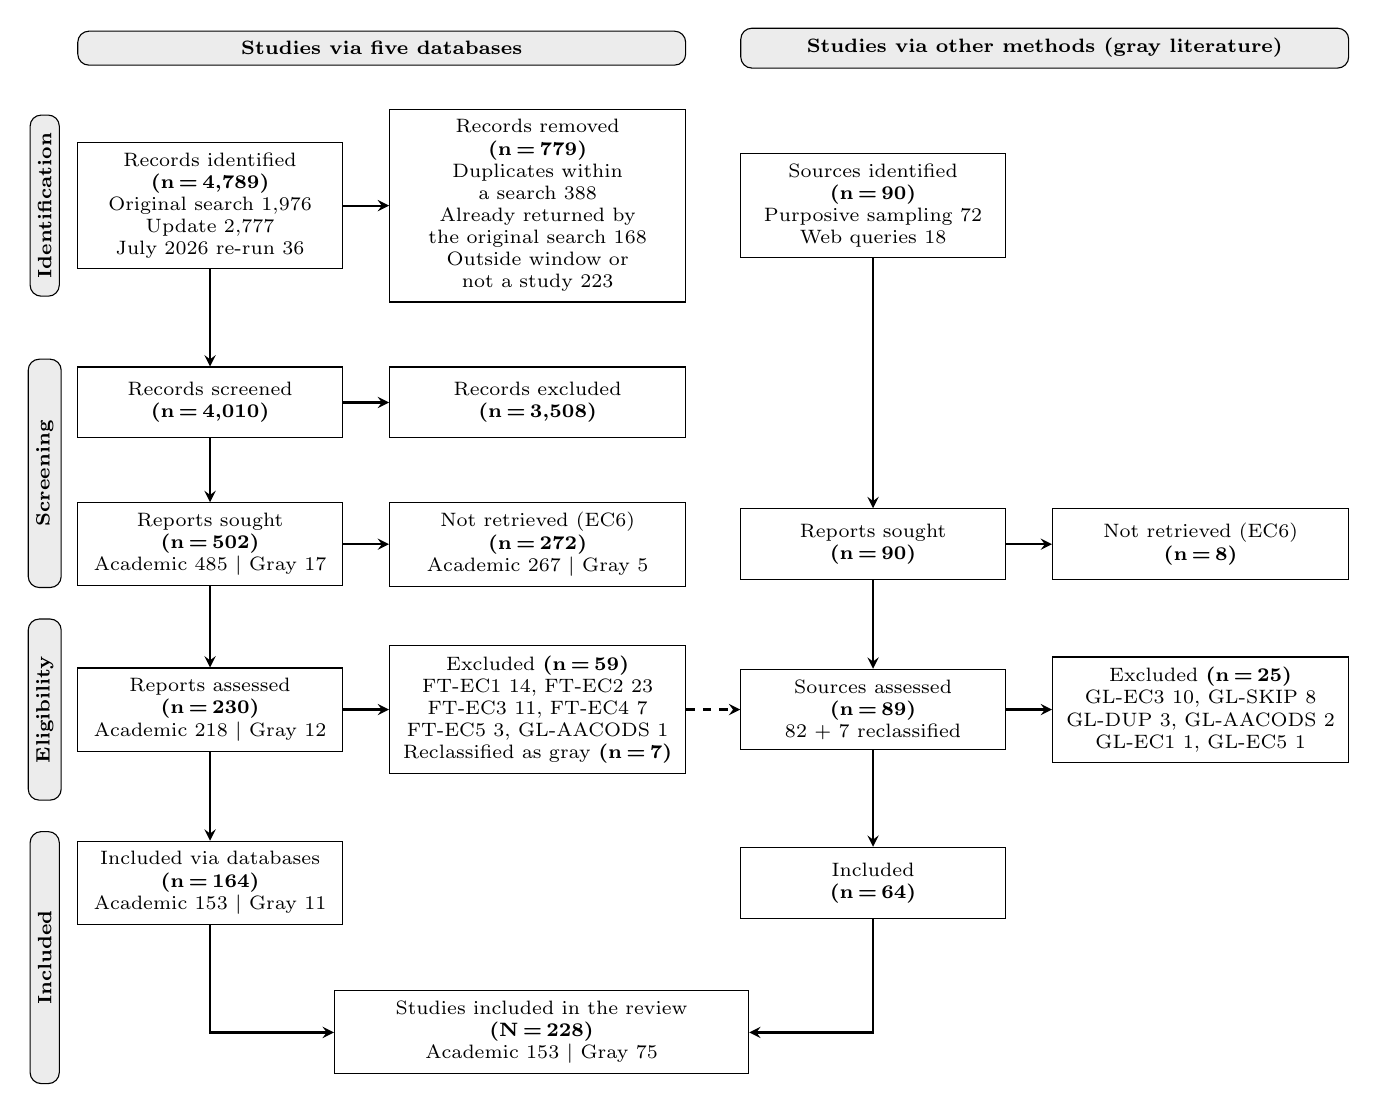
\begin{tikzpicture}[
  every node/.style={font=\scriptsize},
  box/.style={draw, rectangle, align=center, inner sep=1.3mm, minimum height=9mm},
  head/.style={draw, rectangle, rounded corners, align=center, fill=gray!15,
    font=\scriptsize\bfseries, inner sep=1.3mm},
  phase/.style={draw, rectangle, rounded corners, align=center, fill=gray!15,
    font=\scriptsize\bfseries, inner sep=1mm, rotate=90},
  arr/.style={thick, ->, >=stealth},
]
% headers
\node[head, text width=74.6mm] at (21.8mm,4mm) {Studies via five databases};
\node[head, text width=74.6mm] at (106mm,4mm) {Studies via other methods (gray literature)};
% databases
\node[box, text width=31mm] (id) at (0,-16mm)
  {Records identified\\\textbf{(n\,=\,4{,}789)}\\Original search 1{,}976\\Update 2{,}777\\July 2026 re-run 36};
\node[box, text width=35mm] (rem) at (41.6mm,-16mm)
  {Records removed\\\textbf{(n\,=\,779)}\\Duplicates within\\a search 388\\Already returned by\\the original search 168\\Outside window or\\not a study 223};
\node[box, text width=31mm] (scr) at (0,-41mm) {Records screened\\\textbf{(n\,=\,4{,}010)}};
\node[box, text width=35mm] (scrx) at (41.6mm,-41mm) {Records excluded\\\textbf{(n\,=\,3{,}508)}};
\node[box, text width=31mm] (sought) at (0,-59mm) {Reports sought\\\textbf{(n\,=\,502)}\\Academic 485 \textbar\ Gray 17};
\node[box, text width=35mm] (soughtx) at (41.6mm,-59mm) {Not retrieved (EC6)\\\textbf{(n\,=\,272)}\\Academic 267 \textbar\ Gray 5};
\node[box, text width=31mm] (elig) at (0,-80mm) {Reports assessed\\\textbf{(n\,=\,230)}\\Academic 218 \textbar\ Gray 12};
\node[box, text width=35mm] (eligx) at (41.6mm,-80mm)
  {Excluded \textbf{(n\,=\,59)}\\FT-EC1 14, FT-EC2 23\\FT-EC3 11, FT-EC4 7\\FT-EC5 3, GL-AACODS 1\\Reclassified as gray \textbf{(n\,=\,7)}};
\node[box, text width=31mm] (inc) at (0,-102mm) {Included via databases\\\textbf{(n\,=\,164)}\\Academic 153 \textbar\ Gray 11};
% other methods
\node[box, text width=31mm] (gid) at (84.2mm,-16mm) {Sources identified\\\textbf{(n\,=\,90)}\\Purposive sampling 72\\Web queries 18};
\node[box, text width=31mm] (gsought) at (84.2mm,-59mm) {Reports sought\\\textbf{(n\,=\,90)}};
\node[box, text width=35mm] (gsoughtx) at (125.8mm,-59mm) {Not retrieved (EC6)\\\textbf{(n\,=\,8)}};
\node[box, text width=31mm] (gelig) at (84.2mm,-80mm) {Sources assessed\\\textbf{(n\,=\,89)}\\82 + 7 reclassified};
\node[box, text width=35mm] (geligx) at (125.8mm,-80mm)
  {Excluded \textbf{(n\,=\,25)}\\GL-EC3 10, GL-SKIP 8\\GL-DUP 3, GL-AACODS 2\\GL-EC1 1, GL-EC5 1};
\node[box, text width=31mm] (ginc) at (84.2mm,-102mm) {Included\\\textbf{(n\,=\,64)}};
% total
\node[box, text width=50mm] (total) at (42.1mm,-121mm) {Studies included in the review\\\textbf{(N\,=\,228)}\\Academic 153 \textbar\ Gray 75};
% arrows, databases
\draw[arr] (id) -- (rem);
\draw[arr] (id) -- (scr);
\draw[arr] (scr) -- (scrx);
\draw[arr] (scr) -- (sought);
\draw[arr] (sought) -- (soughtx);
\draw[arr] (sought) -- (elig);
\draw[arr] (elig) -- (eligx);
\draw[arr] (elig) -- (inc);
\draw[arr, dashed] (eligx.east) -- (gelig.west);
% arrows, other methods
\draw[arr] (gid) -- (gsought);
\draw[arr] (gsought) -- (gsoughtx);
\draw[arr] (gsought) -- (gelig);
\draw[arr] (gelig) -- (geligx);
\draw[arr] (gelig) -- (ginc);
% to total
\draw[arr] (inc.south) |- (total.west);
\draw[arr] (ginc.south) |- (total.east);
% phase labels
\node[phase, minimum width=23mm] at (-21mm,-16mm) {Identification};
\node[phase, minimum width=29mm] at (-21mm,-50mm) {Screening};
\node[phase, minimum width=23mm] at (-21mm,-80mm) {Eligibility};
\node[phase, minimum width=32mm] at (-21mm,-111.5mm) {Included};
\end{tikzpicture}%
}
\caption{PRISMA 2020 flow diagram of the study selection~\cite{page2021prisma}.}
\label{fig:prisma}
\end{figure}

\subsection{Quality Assessment}
\label{sec:quality}

Academic and gray sources were scored with different checklists. For academic sources, we used six criteria adapted from Dyb{\aa} and Dings{\o}yr~\cite{dyba2008empirical}: clear research objectives, methodological adequacy, description of the sample and context, discussion of threats to validity, sufficient evidence, and contribution to practice or theory. We rated each criterion from 1 to 5, and the quality score is the mean of the six. For gray literature, we used the six criteria of Garousi et al.~\cite{garousi2019mlr}, based on AACODS, namely the authority of the author or organization, the rigor of the method description, currency, objectivity and declared commercial interest, references to external evidence, and novelty. We rated each criterion from 1 to 6, and the quality score is again the mean of the six. Neither checklist prescribes a cut-off score, so we chose the minimum. We set it at 3.0 on both scales, which is the midpoint of the academic scale and half a point below the midpoint of the gray scale. An academic full text below this minimum was excluded under FT-EC3 unless another exclusion criterion applied first; for gray sources, the minimum served as an inclusion gate (GL-AACODS).

In the original search, the first author manually scored every source, and each structured reading form records the score and a supporting quote from the full text~\cite{replication2026}. The ratings that Claude and NotebookLM produced during extraction, on a different scale, served only as a reference, and the final score is the first author's. 

In the update, Claude drafted the scores of 117 of the 127 assessed sources, criterion by criterion, each with a short justification and a page reference. The drafts were calibrated against the first author's per-criterion scores in the original corpus. The first author checked every draft against the full text, agreed with all of them, and scored the other ten sources directly. The ratings of the two extractors diverged beyond the comparison tolerance in 52 of the 106 academic and 12 of the 30 gray update sources, so neither was used as a score.

The 153 included academic sources had a mean score of 4.19/5.0 (SD\,=\,0.61), with 23 at 5.0, 83 between 4.0 and 4.99, and 47 between 3.0 and 3.99. No included source scored below 3.0 because quality was assessed during full-text reading, and full texts below this minimum were excluded under FT-EC3 (Section~\ref{sec:selection}). This criterion excluded 11 full texts: 5 from the original search and 6 from the update. Two of the six update exclusions scored below 3.0, and the other four rest on data that could not be traced, regardless of their score.

The 75 included gray sources had a mean score of 4.27/6.0 (SD\,=\,1.04), with 18 sources at exactly 3.0 and 11 at the maximum of 6.0. Not every gray candidate was included. In the original search, 55 of the 79 gray sources assessed were included, and in the update, 20 of the 22. Figure~\ref{fig:prisma} explains each exclusion. One of the two excluded in the update scored 2.0/6.0, and the other, above the minimum, was excluded under GL-AACODS because its reported data were not credible.

We also graded the strength of the evidence behind each academic source, with levels adapted from Razzaq et al.~\cite{P0604}. A source's findings rest on questionnaires when they come from questionnaire or survey data, and they are substantiated when they come from a positivist evaluation, such as measurement, an experiment, or repository analysis. Reviews rest on secondary synthesis, and a source is graded as a mention or a conceptual proposal when its findings are not backed by its own data. By this grading, 65 academic sources rest on questionnaires, 61 on substantiated evaluation, 15 on secondary syntheses, 10 on mentions, and 2 on conceptual proposals. The grading differs from the research method in Table~\ref{tab:study_char}. A mixed-methods study whose main findings come from a survey, for example, counts as a mixed-methods design and as resting on questionnaires, which is why the 65 questionnaire-based sources outnumber the 29 survey studies.

\subsection{Data Extraction}
\label{sec:extraction}

We used two LLM-based assistants for data-extraction triangulation, following Felizardo et al.~\cite{felizardo2024llm}. Claude (Anthropic) and NotebookLM (Google) independently extracted each source with the same structured zero-shot prompt, which instructed them to report only what the source states and not to infer. As Felizardo et al.\ recommend, we reconciled the LLM output with human extraction rather than replacing it. The first author compared both outputs with the full text and decided every field, and other authors reviewed these decisions (Section~\ref{sec:second-reviewer}). The authors always made selection decisions, and the extractors' verdicts served only as an audit signal. The extraction form, defined \textit{a priori} and available in the replication package~\cite{replication2026}, covers bibliographic data, study characterization, metrics and frameworks, productivity factors, the role of AI, the quality criteria (Section~\ref{sec:quality}), and the contributions and limitations reported by the authors.

In the original search, the two extractors processed the 139 full texts available at that point (110 academic and 29 gray), before the final eligibility and reclassification decisions. All 66 included academic studies are among them, and the first author coded eight late gray additions directly, including the seven sources reclassified from the academic set. A script compared the two outputs field by field and classified each pair as an exact match (identical or equivalent values), a partial match (overlapping values, one more specific than the other, such as ``Survey'' and ``Survey + Interviews''), or divergent. Table~\ref{tab:concordance} reports the concordance for seven fields. Its categorical rows count only the sources for which both extractors returned a value, 89 for study type, 53 for research method, and 62 for context. 

The comparison flagged 298 field-level discrepancies, all of which the first author resolved by rereading the full text, choosing the more accurate value in 267 cases and correcting 31 false divergences caused by synonyms. Against the final coding, Claude matched 96.4\% of the binary classifications and NotebookLM 94.2\%, while for the categorical fields the rates were 38.1\% and 31.7\%, respectively. The categorical fields diverged mostly in vocabulary and granularity. As an example, for a longitudinal study~\cite{P0485}, Claude reported ``computer monitoring with experience sampling'' and NotebookLM a ``mixed-methods study with surveys and interviews''. Some disagreements were substantive. Claude classified a study that proposes a method based on COSMIC function points~\cite{P0030} as a randomized controlled trial, and it marked ten studies that NotebookLM marked as using SPACE as not using SPACE, such as Li et al.~\cite{P1303}, whose use of SPACE the first author confirmed. In such cases, the first author coded the field from the full text, and the resolution log is in the replication package~\cite{replication2026}.

\begin{table}[htbp]
\centering
\caption{Agreement between Claude and NotebookLM in the original search ($n$\,=\,139).}
\label{tab:concordance}
\footnotesize
\begin{tabular}{l c c c c c}
\toprule
\textbf{Field} & \textbf{Exact} & \textbf{Partial} & \textbf{Divergent} & \textbf{Agree\%} & \textbf{Post-resol.} \\
\midrule
\multicolumn{6}{l}{\textit{Binary classification fields}} \\
\quad DORA used     & 131 & 0  & 8   & 94.2\% & 100\% \\
\quad SPACE used    & 129 & 0  & 10  & 92.8\% & 100\% \\
\quad AI discussed  & 92  & 0  & 47  & 66.2\% & 100\% \\
\midrule
\multicolumn{6}{l}{\textit{Categorical fields}} \\
\quad Study type       & 14  & 10 & 65  & 27.0\% & 100\% \\
\quad Research method  & 24  & 0  & 29  & 45.3\% & 100\% \\
\quad Context          & 12  & 0  & 50  & 19.4\% & 100\% \\
\midrule
\multicolumn{6}{l}{\textit{Count-based fields}} \\
\quad Metrics count    & 44  & 9  & 86  & 38.1\% & 100\% \\
\bottomrule
\end{tabular}
\end{table}

In the update, the 136 sources with retrieved full text (106 academic and 30 gray) went through the same two extractors with the same prompt. Claude Opus 5.5 replaced the Claude Opus 4.8 used in the original search, and each update extraction file records the model version. NotebookLM does not disclose its underlying model. The automatic comparison covered 1{,}664 field-level pairs: 35.4\% were exact matches, 29.4\% partial matches, 22.9\% divergent, and 12.3\% missing a value from at least one extractor. For the academic sources, the extractors agreed that DORA, SPACE, and DevEx were used to measure in 96.2\%, 93.4\%, and 93.4\% of cases, respectively. Unlike in the original corpus, the reading forms of the update came pre-filled. A field was filled only when both extractors returned the same value, and every filled value carried a verbatim passage and its page, which the script checked against the full text. 

This filled 1{,}894 of the 2{,}082 fields (91.0\%), and the first author checked every field against the full text. Claude drafted the remaining fields of the included sources (166 fields in 90 sources) from the full text, and the first author approved them. The first author drafted fields the update form did not contain (strength of evidence and sample size for academic sources, and DevEx engagement level, tier, and vendor classification for gray sources) in the same way and reviewed them. The eligibility decision and the exclusion criterion were never pre-filled. Both extractors returned Include for all 136 sources, and the first author excluded 29 of them: 9 under EC6 because only a partial or different version of the text was available, and 20 at eligibility.

For each framework, we coded two ways in which an academic source can engage with it. A source uses the framework as its measurement instrument when it operationalizes the framework's constructs to collect or analyze its own data, in accordance with the framework's formal proposal. A source cites the framework when it names it in its background, motivation, or discussion. Every source that uses a framework also cites it, and in DevEx, citations include references to developer experience as a construct. Section~\ref{sec:rq1} gives examples of both. For each gray source, we coded the engagement with each framework at three levels. A gray source uses a framework to measure real teams, organizations, or repositories with the framework's constructs; provides guidance or commentary when it defines, teaches, compares, or critiques the framework without measuring it; and cites the framework only when it appears in a role other than measurement. We identified mentions via full-text search across the gray corpus, and the coding sheets are included in the replication package~\cite{replication2026}.

Every source, academic and gray, was coded against nine metric categories. A codebook defines each category with inclusion and exclusion rules, summarized in Table~\ref{tab:metric_taxonomy} (Section~\ref{sec:rq1}). The coding is multi-label, and each positive flag requires a supporting quote from the source. The extraction form also recorded the name of every concrete metric each source reports. We normalized these names to canonical metrics with rule-based matching and manual curation. The codebook and the resulting metric list are in the replication package~\cite{replication2026}.

\subsection{Data Synthesis}
\label{sec:synthesis}

We combined quantitative and qualitative analysis to answer the four research questions. Quantitatively, we tabulated citations, framework use, metric categories, and their distributions across the three periods (2016--2019, 2020--2022, and 2023--2026) in the extraction data. We compared academic and gray sources with Fisher's exact test for each framework and a chi-square test for the use of any framework, and we report these tests as descriptive aids (Section~\ref{sec:threats}). Qualitatively, we used open coding~\cite{strauss1998basics} to identify measurement challenges, contextual factors, and anti-patterns, following Trinkenreich et al.~\cite{trinkenreich2022women}. In the original search, we attached codes to quoted passages in each source and iteratively grouped them into themes (Table~\ref{tab:challenges}). In the October 2026 update, we recoded the challenges across all academic sources using the codebook developed through this open coding process. Claude drafted the codes for each source, including a quote and the page number from the full text, and the first author checked them. Other authors then reviewed the codes and themes, and the authors involved discussed disagreements in meetings until they reached consensus (Section~\ref{sec:second-reviewer}).

\subsection{Expert Review and Validation}
\label{sec:second-reviewer}
The first author carried out the selection, extraction, and quality assessment. Other authors therefore independently reviewed the complete set of decisions, which covers the inclusion and exclusion criteria, all classifications, and the quality and evidence grading. They examined the original full texts alongside each decision, and the authors involved resolved disagreements by consensus. The same review covered the search update decisions.

% ============================================================
% 4. RESULTS
% ============================================================

\section{Results}
\label{sec:results}

We first describe the included studies and then report the results for each research question. The final corpus comprises 228 sources, 153 academic studies (67.1\%) and 75 gray literature sources (32.9\%), summarized in Table~\ref{tab:overview}. The original search contributed 121, and the October 2026 update contributed 107.

\subsection{Overview of the Included Studies}
\label{sec:overview}

\begin{table}[htbp]
\centering
\caption{Overview of the included sources.}
\label{tab:overview}
\footnotesize
\begin{tabular}{l r r}
\toprule
\textbf{Characteristic} & \textbf{Academic} & \textbf{Gray Lit.} \\
\midrule
\rowcolor{lightgray}
Total sources & 153 & 75 \\
\quad Original search (Jan--Feb 2026) & 66 & 55 \\
\quad Search update (Oct 2026) & 87 & 20 \\
By period & & \\
\quad Pre-pandemic (2016--2019) & 19 & 2 \\
\quad Pandemic (2020--2022) & 25 & 6 \\
\quad Post-pandemic/AI (2023--2026) & 109 & 67 \\
\rowcolor{lightgray}
Gray literature tier & & \\
\quad 1st tier (high authority) & n/a & 29 \\
\quad 2nd tier (moderate) & n/a & 41 \\
\quad 3rd tier (practitioner) & n/a & 5 \\
\bottomrule
\end{tabular}
\end{table}

The academic sources were published mostly at conferences (92, 60.1\%) and in journals (52, 34.0\%). Mixed-methods designs (35, 22.9\%) and surveys (29, 19.0\%) were the most common of the ten research methods (Table~\ref{tab:study_char}). Of the 98 academic sources that collected data from participants, the median sample size is 54.5, and 35 have samples below 30.

\begin{table}[htbp]
\centering
\caption{Characterization of the academic studies ($n$\,=\,153).}
\label{tab:study_char}
\footnotesize
\begin{tabular}{l r r | l r r}
\toprule
\textbf{Publication Venue} & \textbf{$n$} & \textbf{\%} & \textbf{Research Method} & \textbf{$n$} & \textbf{\%} \\
\midrule
Conference Paper     & 92 & 60.1 & Mixed Methods            & 35 & 22.9 \\
Journal Article      & 52 & 34.0 & Survey                   & 29 & 19.0 \\
Workshop Paper       & 8  & 5.2  & Conceptual / Other       & 16 & 10.5 \\
Thesis               & 1  & 0.7  & Repository Mining        & 15 & 9.8  \\
                     &    &      & Review / Secondary       & 14 & 9.2  \\
                     &    &      & Case Study               & 13 & 8.5  \\
                     &    &      & Qualitative / Interviews & 12 & 7.8  \\
                     &    &      & Controlled Experiment    & 10 & 6.5  \\
                     &    &      & Experience Report        & 7  & 4.6  \\
                     &    &      & Quasi-Experiment         & 2  & 1.3  \\
\bottomrule
\end{tabular}
\end{table}

\subsection{RQ1. Frameworks, metrics, and tools}
\label{sec:rq1}

In this section, we present results that address RQ1: \textit{What frameworks, metrics, and tools have been used to measure software developer productivity in academic and practitioner literature from 2016 to 2026?} 

\subsubsection{Framework Citation and Use}

We distinguish sources that use a framework, operationalizing its constructs to collect or analyze their own data, from sources that only cite it (Section~\ref{sec:extraction}). R\"uegger et al.~\cite{P0470}, for example, built a tool that computes the four DORA metrics for 37 microservices, and Fortes et al.~\cite{P0244} measured the three DevEx dimensions to model the perceived productivity of 106 developers. Chen et al.~\cite{P2100}, in contrast, cite DORA, SPACE, and the framework of Greiler et al., but build their own six-factor framework from a survey of 2,989 developers. Sources that only cite a framework are in the corpus because of their own measurement contribution (IC2), so the citation counts below describe this corpus rather than the literature at large.

Among the 153 academic studies, DORA is cited in 19 and used in 9, SPACE is cited in 49 and used in 19, and DevEx is cited in 37 and used in 12 (Table~\ref{tab:acad_vs_gl}, Figure~\ref{fig:framework_flow}). SPACE is the most used framework (19 studies, 12.4\%)~\cite{P1259, P0001, P1816, P0112, P0061, P0549, P1261, P1476, P1303, P0181, P2019, P2020, P2038, P2041, P2059, P2073, P2131, P2133, P2134}. The DevEx framework of Noda et al.\ follows (12 studies, 7.8\%)~\cite{P1280, P1356, P0021, P0593, P0001, P0244, P1261, P2015, P2019, P2073, P2079, P2080}, and then DORA (9 studies, 5.9\%)~\cite{P0470, P0003, P1261, P2008, P2013, P2014, P2017, P2026, P2043}. In total, 35 of the 153 academic studies (22.9\%) use at least one of the three frameworks, 31 of them one framework and four use two or more. The other 118 studies measure productivity without one of these frameworks. Of these 118, 86 (72.9\%) use study-specific survey instruments, 71 (60.2\%) use satisfaction measures, and 77 (65.3\%) use direct productivity or performance measures.

Gray sources engage with the frameworks at three levels (Table~\ref{tab:acad_vs_gl}, Figure~\ref{fig:framework_flow}). DORA is the framework most often used to measure (12 of 75 sources, 16.0\%)~[\refG{G004}, \refG{G009}, \refG{G046}, \refG{G074}, \refG{G115}], followed by SPACE (10, 13.3\%)~[\refG{G009}, \refG{G014}, \refG{G046}, \refG{G082}, \refG{G091}] and DevEx (5, 6.7\%)~[\refG{G022}, \refG{G077}, \refG{G078}, \refG{G092}]. Guidance or commentary is the most common engagement with DORA (24 sources) and DevEx (15), and another 15 and 10 sources only cite them. For SPACE, citation-only mentions (15) outnumber guidance (13). In total, 64 of the 75 gray sources (85.3\%) cite at least one framework, and 23 (30.7\%) use at least one to measure. The use of DORA to measure concentrates in sources produced by vendors or framework maintainers, with 30.3\% of these 33 sources against 4.8\% of the 42 independent ones (Section~\ref{sec:threats}).

Only for DORA do the communities differ, with use measured in 12 of 75 gray sources versus 9 of 153 academic studies (Fisher's exact $p$\,=\,0.026). The differences for SPACE and DevEx are not significant ($p$\,=\,0.84 and $p$\,=\,1.00), and neither is the difference in the use of any of the three frameworks (30.7\% of gray against 22.9\% of academic sources, $\chi^2$\,=\,1.23, $p$\,=\,0.27). We ran these four tests without correcting for multiple comparisons, and the DORA result does not survive a Bonferroni correction across the three framework tests ($p$\,=\,0.077). We therefore treat it as a difference worth describing rather than an established one, especially since Section~\ref{sec:threats} traces it to vendor and maintainer sources.

\begin{table}[htbp]
\centering
\caption{Framework citation and use by community.}
\label{tab:acad_vs_gl}
\footnotesize
\setlength{\tabcolsep}{3.5pt}
\begin{tabular}{l c c c c c}
\toprule
 & \multicolumn{2}{c}{\textbf{Academic ($n$\,=\,153)}} & \multicolumn{3}{c}{\textbf{Gray ($n$\,=\,75)}} \\
\cmidrule(lr){2-3}\cmidrule(lr){4-6}
\textbf{Framework} & \textbf{Cited} & \textbf{Used} & \textbf{Used to measure} & \textbf{Guidance} & \textbf{Cited only} \\
\midrule
DORA  & 19 (12.4\%) & 9 (5.9\%)   & 12 (16.0\%) & 24 (32.0\%) & 15 (20.0\%) \\
SPACE & 49 (32.0\%) & 19 (12.4\%) & 10 (13.3\%) & 13 (17.3\%) & 15 (20.0\%) \\
DevEx & 37 (24.2\%) & 12 (7.8\%)  & 5 (6.7\%)   & 15 (20.0\%) & 10 (13.3\%) \\
\bottomrule
\end{tabular}
\end{table}

\begin{figure}[htbp]
\centering
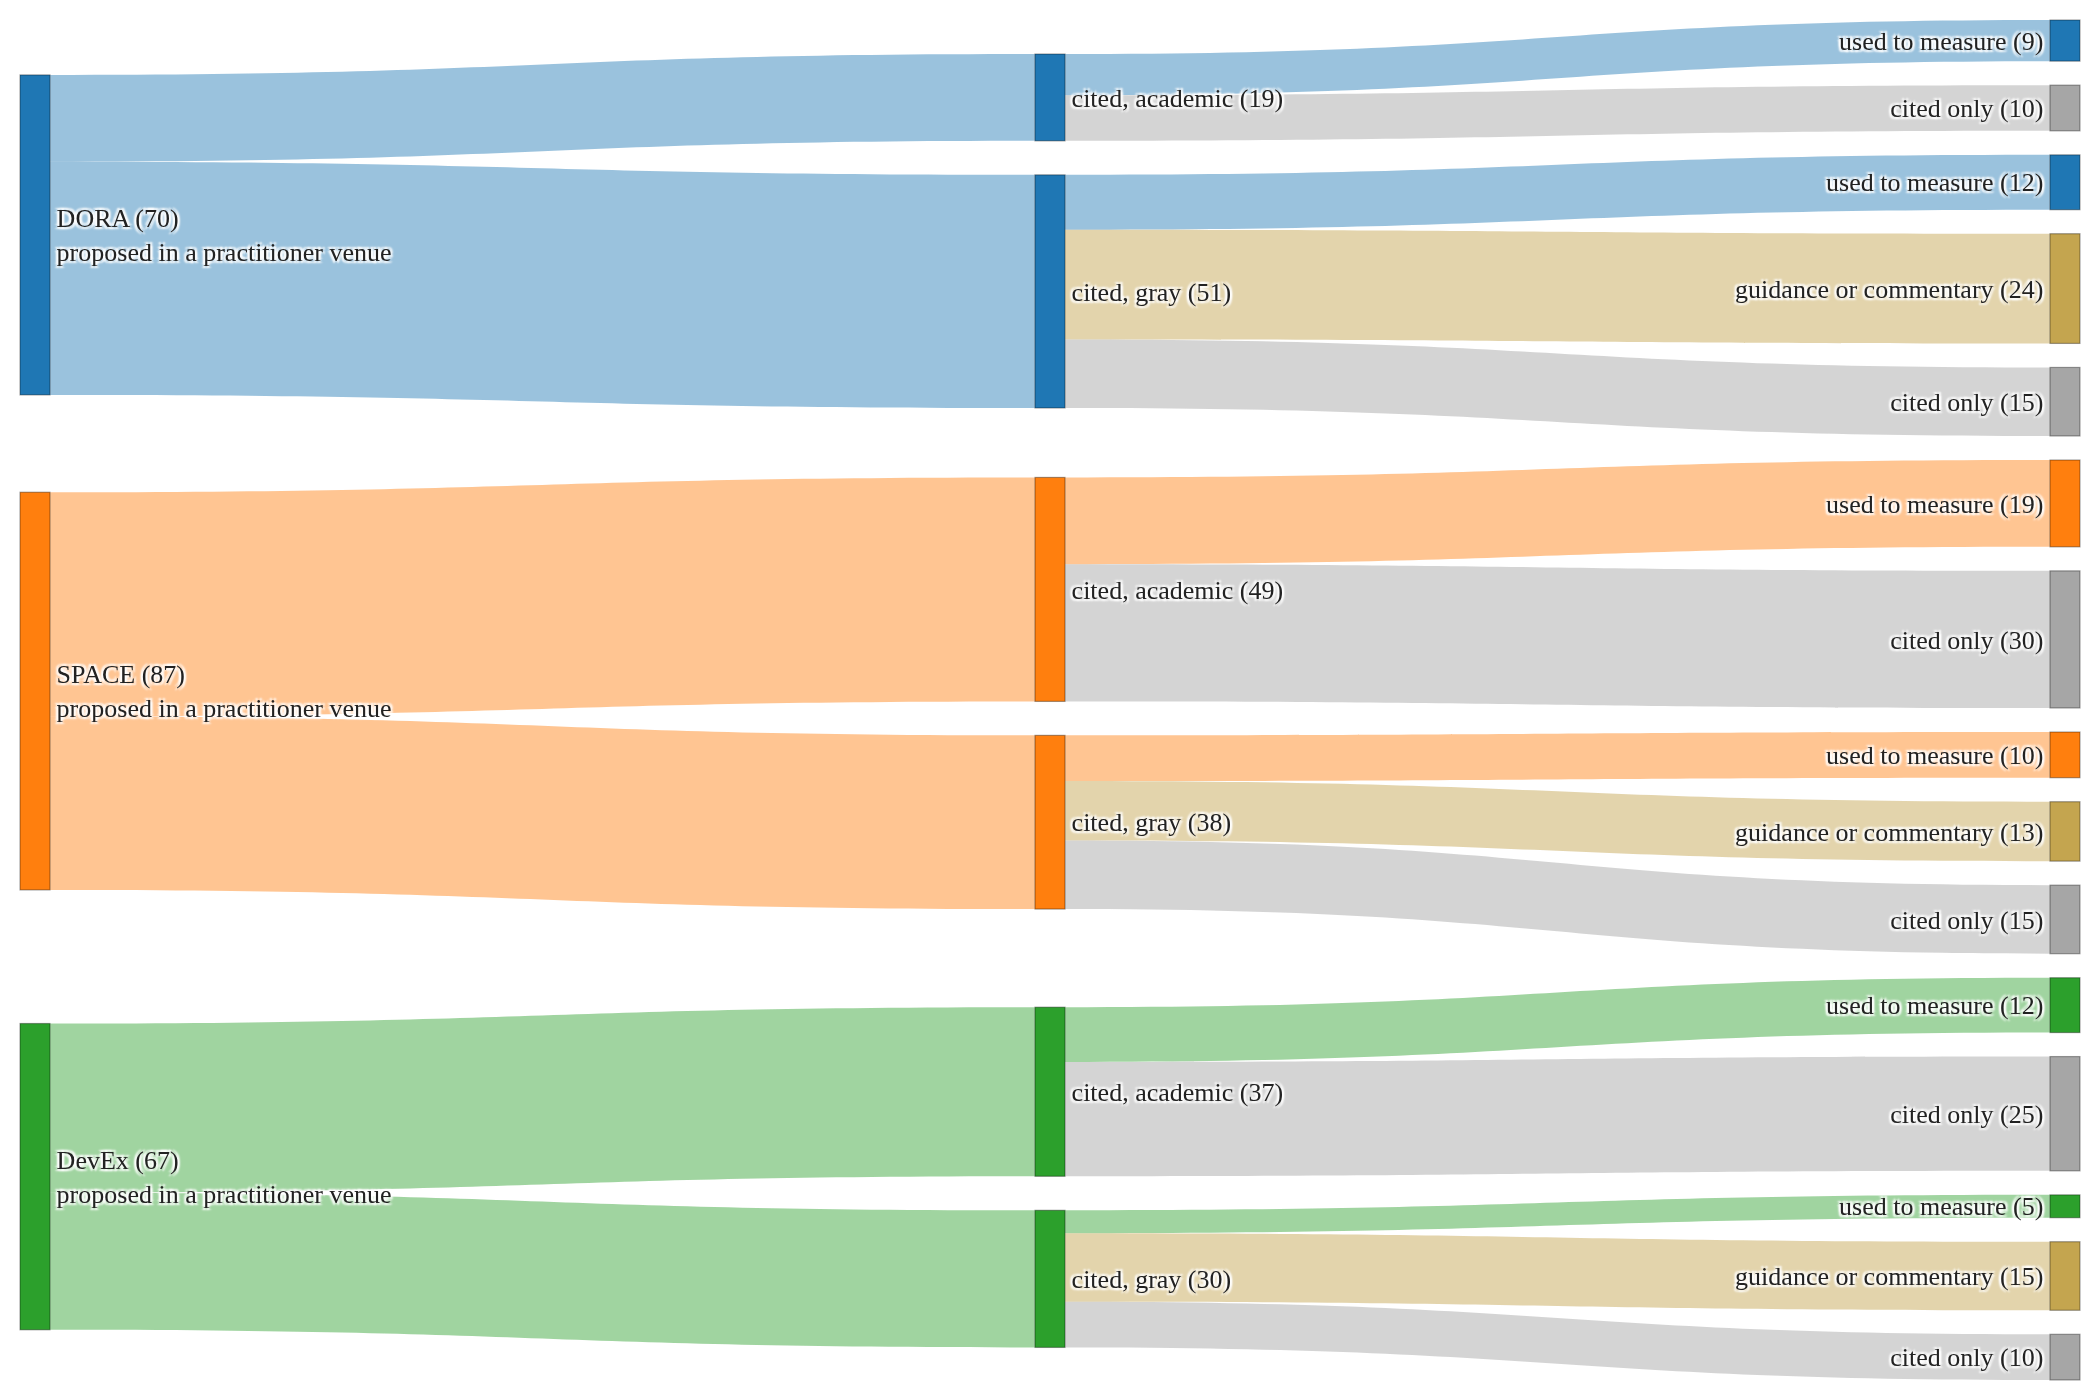
\includegraphics[width=\textwidth]{figures/fig_framework_flow.png}
\caption{Citation and use of DORA, SPACE, and DevEx ($N$\,=\,228).}
\label{fig:framework_flow}
\end{figure}

\subsubsection{Metric Categories}

Table~\ref{tab:metric_taxonomy} defines the nine metric categories of the codebook and gives example metrics, example studies, and the number of sources in each community. The categories are not mutually exclusive at the source level, since a source is flagged in every category it measures, and survey or perceptual measurement describes how a construct is measured rather than which one. At the metric level, each of the 62 metrics in Supplementary Table S3 belongs to a single category. Across the 228 sources, survey and perceptual measures were the most frequent (168 sources, 73.7\%), followed by productivity and performance metrics (163, 71.5\%) and satisfaction and well-being metrics (143, 62.7\%). Quality metrics appeared in 128 sources (56.1\%), collaboration metrics in 113 (49.6\%), and activity metrics in 104 (45.6\%). Delivery performance (74, 32.5\%), agile and process metrics (69, 30.3\%), and the DevEx dimensions (32, 14.0\%) were the least frequent. Each source addresses, on average, 4.4 of the nine categories, and only nine sources (3.9\%) rely on a single category. Perceptual, productivity, and satisfaction metrics appear together in 92 sources (40.4\%). The communities differ most in delivery performance, which appears in 62.7\% of the gray sources and 17.6\% of the academic studies. In the academic studies, satisfaction and well-being appear in 62.1\% of the sources and collaboration in 45.8\%. Of the 74 sources that report delivery performance metrics, 59 also report satisfaction, collaboration, or DevEx metrics (20 of the 27 academic and 39 of the 47 gray sources). %Remote or COVID-specific measurement appears in 10.1\% of all sources.

\begin{table}[htbp]
\centering
\caption{Metric categories of the codebook, with $n$ (\%) of sources.}
\label{tab:metric_taxonomy}
\scriptsize
\setlength{\tabcolsep}{2pt}
\begin{tabular}{>{\raggedright\arraybackslash}p{2.05cm} >{\raggedright\arraybackslash}p{2.95cm} >{\raggedright\arraybackslash}p{2.1cm} >{\raggedright\arraybackslash}p{1.02cm} >{\centering\arraybackslash}p{0.95cm} >{\centering\arraybackslash}p{0.95cm} >{\centering\arraybackslash}p{0.95cm}}
\toprule
\textbf{Category} & \textbf{Definition} & \textbf{Example metrics} & \textbf{Studies} & \textbf{Acad.} & \textbf{Gray} & \textbf{Total} \\
\midrule
Survey / Perceptual & Perceptions collected with surveys, self-reports, or interviews & self-reported productivity, perceived efficiency & \cite{P0321, P0249} & 115\newline(75.2) & 53\newline(70.7) & 168\newline(73.7) \\
\addlinespace
Productivity / Performance & Output or performance, except perceived productivity and delivery & velocity, throughput, task completion time & \cite{P0017, P0027} & 100\newline(65.4) & 63\newline(84.0) & 163\newline(71.5) \\
\addlinespace
Satisfaction / Well-being & Satisfaction, engagement, stress, and well-being & job satisfaction, burnout, work-life balance & \cite{P0529, P0534} & 95\newline(62.1) & 48\newline(64.0) & 143\newline(62.7) \\
\addlinespace
Quality & Quality and stability of the code and the system & defects, change failure rate, test coverage & \cite{P0271, P0556} & 72\newline(47.1) & 56\newline(74.7) & 128\newline(56.1) \\
\addlinespace
Collaboration & Communication and coordination, except commit counts & code review, knowledge sharing, meetings & \cite{P1503, P0162} & 70\newline(45.8) & 43\newline(57.3) & 113\newline(49.6) \\
\addlinespace
Activity / Code & Raw counts of repository activity & commits, pull requests, lines changed & \cite{P0162, P0481} & 58\newline(37.9) & 46\newline(61.3) & 104\newline(45.6) \\
\addlinespace
Delivery Performance & Speed and frequency of delivery & deployment frequency, lead time, cycle time & \cite{P0003, P0470} & 27\newline(17.6) & 47\newline(62.7) & 74\newline(32.5) \\
\addlinespace
Agile / Process & Agile ceremonies, workflow, and planning & sprint metrics, kanban flow, iteration cadence & \cite{P0017, P0178} & 33\newline(21.6) & 36\newline(48.0) & 69\newline(30.3) \\
\addlinespace
DevEx Dimensions & Explicit use of the DevEx framework & flow state, cognitive load, feedback loops & \cite{P1280, P0244} & 12\newline(7.8) & 20\newline(26.7) & 32\newline(14.0) \\
\bottomrule
\end{tabular}
\end{table}

\subsubsection{List of Metrics}

Beyond the categories, the extraction forms record the concrete metrics that each source reports. After normalization, 62 canonical metrics in the nine categories cover 223 sources. The list assigns each canonical metric to one category but is coded independently of the category flags. Flow state, for example, is listed under the DevEx dimensions and appears in 39 sources, whereas the DevEx category flags only the 32 sources that use the DevEx framework itself. Supplementary Table S3 lists the 62 metrics and their sources, and Figure~\ref{fig:metric_inventory} shows the 15 most-reported metrics by community. Perceived productivity led with 49 sources~\cite{P0249, P0112}, followed by composite productivity scores with 48~\cite{P0017}~[\refG{G014}], and by lines of code changed~\cite{P0162} and code quality or health~\cite{P0271, P2032} with 45 sources each. Task or contribution throughput and developer satisfaction appeared in 44 sources each, and task completion time in 42~\cite{P2029, P0485}.

The communities report different metrics. The DORA delivery metrics appear mostly in gray sources, with deployment frequency in 23 gray and 9 academic sources~\cite{P0470}~[\refG{G001}], change failure rate in 16 and 9~\cite{P0003}~[\refG{G017}], and mean time to restore in 13 and 8. Academic studies more often report self-reported and affective measures. Perceived productivity appears in 43 academic sources versus six gray sources~\cite{P0249, P0112}, and affect or sentiment measures appear in 16 academic sources and one gray source~\cite{P0529, P0534}. Metrics specific to AI-assisted development, such as suggestion acceptance and code persistence, appear in 28 sources (20 academic and 8 gray)~\cite{P0549}~[\refG{G014}]. Of these, 26 were published in 2024 or later.

\begin{figure}[htbp]
\centering
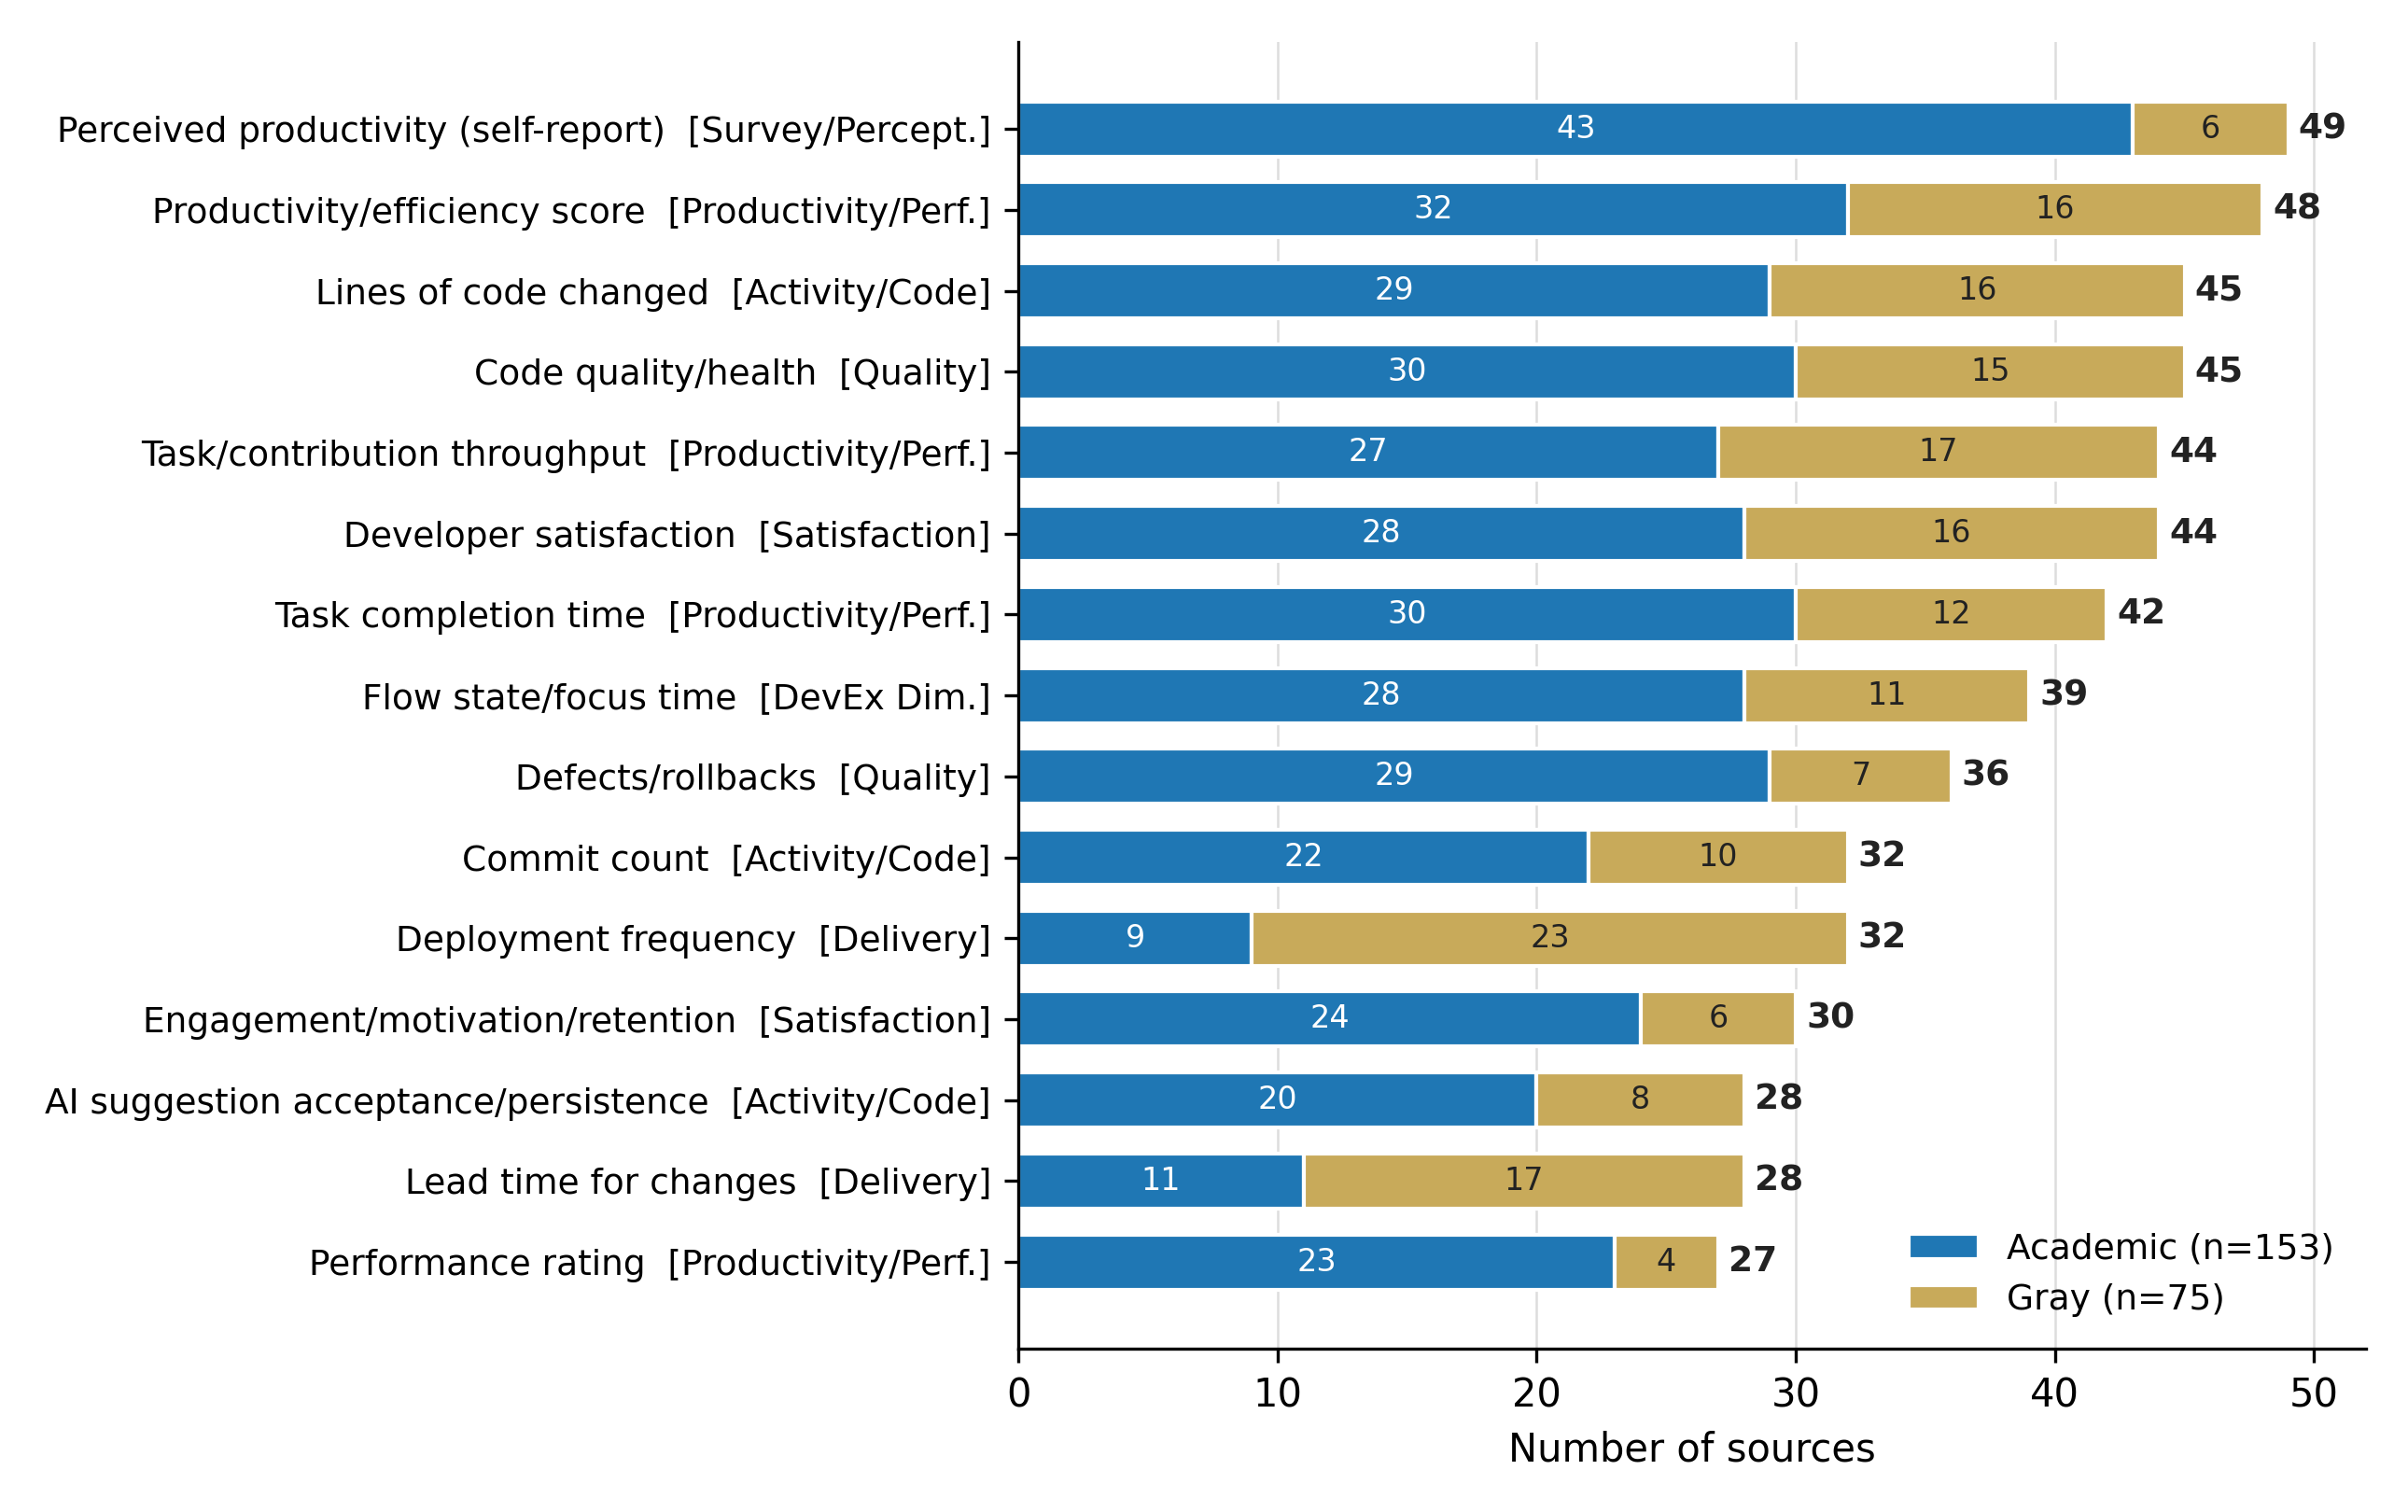
\includegraphics[width=\textwidth]{figures/fig_metric_inventory.png}
\caption{Fifteen most reported metrics by community.}
\label{fig:metric_inventory}
\end{figure}

\begin{tcolorbox}[colback=gray!5, colframe=gray!50, title={\textbf{Summary of RQ1}}, fonttitle=\small]
\footnotesize
In academic studies, the frameworks are cited far more often than they are used as measurement instruments. SPACE is used in 19 studies (12.4\%), DevEx in 12 (7.8\%), and DORA in 9 (5.9\%), and 22.9\% of the studies use at least one. Most gray sources cite a framework (85.3\%), mostly through guidance, commentary, or citation only. Use of DORA for measurement is more frequent in gray sources only (16.0\% vs. 5.9\%), and that gap is concentrated in vendor and maintainer sources (30.3\% vs. 4.8\% for independent gray sources). Across the 228 sources, the most common metric categories are perceptual measures (73.7\%), productivity and performance (71.5\%), and satisfaction and well-being (62.7\%). Each source covers, on average, 4.4 of the nine categories.
\end{tcolorbox}

\subsection{RQ2. Temporal evolution}
\label{sec:rq2}

In this section, we present the results that support the answer to RQ2: \textit{How has developer productivity measurement evolved across the pre-pandemic, pandemic transition, and post-pandemic/AI era?}

The number of academic papers grew across the periods, with 19 in 2016--2019, 25 in 2020--2022, and 109 in 2023--2026 (Table~\ref{tab:temporal_detail}). The update added 87 of them, 74 from 2023--2026 and 13 from earlier years, 11 of which came from the candidates of the July 2026 Google Scholar re-run. Of the 75 gray sources, 67 (89.3\%) appeared in 2023--2026~[\refG{G004}, \refG{G009}, \refG{G022}, \refG{G027}, \refG{G036}, \refG{G040}, \refG{G046}, \refG{G047}, \refG{G048}, \refG{G092}, \refG{G099}, \refG{G115}].

The use of the frameworks as measurement instruments falls almost entirely in the most recent period (Table~\ref{tab:temporal_detail}). All nine academic DORA uses~\cite{P0003, P0470, P1261, P2017} and all twelve DevEx uses fall in 2023--2026, as do 16 of the 19 SPACE uses. The other three SPACE uses date from 2021 and 2022~\cite{P1259, P0061, P0549}, and no academic study used any of the three frameworks before 2020. With no use before 2020 and at most three uses per framework in 2020--2022, the counts are too small to test the differences between periods for each framework.

\begin{table}[htbp]
\centering
\caption{Key indicators by period.}
\label{tab:temporal_detail}
\footnotesize
\begin{tabular}{l c c c}
\toprule
\textbf{Indicator} & \textbf{Pre-pand.} & \textbf{Pandemic} & \textbf{Post-pand.} \\
 & \textbf{(2016--19)} & \textbf{(2020--22)} & \textbf{(2023--26)} \\
\midrule
\multicolumn{4}{l}{\textit{Source counts}} \\
\quad Academic papers & 19 & 25 & 109 \\
\quad Gray literature & 2  & 6  & 67 \\
\midrule
\multicolumn{4}{l}{\textit{Framework used as measurement instrument (academic)}} \\
\quad DORA  & 0 & 0 & 9 \\
\quad SPACE & 0 & 3 & 16 \\
\quad DevEx & 0 & 0 & 12 \\
\midrule
\multicolumn{4}{l}{\textit{Emerging themes (academic)}} \\
\quad Remote/hybrid studies & 0 & 8 & 12 \\
\quad AI-related studies  & 0 & 1 & 60 \\
\bottomrule
\end{tabular}
\end{table}

Table~\ref{tab:cat_period} shows the share of academic sources reporting each of the nine metric categories and remote-specific measurement in each period. Three movements stand out. Activity metrics jumped from 5\% of studies in 2016--2019 to 52\% in 2020--2022, then settled at 40\% afterward, and collaboration rose from 26\% to 48\% and stayed at 49\%. Quality (16\%, 24\%, 58\%), delivery performance (5\%, 4\%, 23\%), and productivity and performance (58\%, 56\%, 69\%) rose only after 2022, and the DevEx dimensions appear in that period alone (11\%). Satisfaction and well-being (53\%, 64\%, 63\%), survey or perceptual measurement (79\%, 60\%, 78\%), and agile and process metrics (21--24\%) stayed within a narrow band throughout. Remote or COVID-specific measurement appears in 32\% of the pandemic-period studies and in 11\% of those from 2023--2026.


\begin{table}[htbp]
\centering
\caption{Metric categories in academic sources by period, $n$ (\%).}
\label{tab:cat_period}
\footnotesize
\begin{tabular}{l c c c}
\toprule
\textbf{Category} & \textbf{2016--2019} & \textbf{2020--2022} & \textbf{2023--2026} \\
 & \textbf{($n$\,=\,19)} & \textbf{($n$\,=\,25)} & \textbf{($n$\,=\,109)} \\
\midrule
Survey / Perceptual        & 15 (79) & 15 (60) & 85 (78) \\
Productivity / Performance & 11 (58) & 14 (56) & 75 (69) \\
Satisfaction / Well-being   & 10 (53) & 16 (64) & 69 (63) \\
Quality                    & 3 (16)  & 6 (24)  & 63 (58) \\
Collaboration              & 5 (26)  & 12 (48) & 53 (49) \\
Activity / Code            & 1 (5)   & 13 (52) & 44 (40) \\
Delivery Performance       & 1 (5)   & 1 (4)   & 25 (23) \\
Agile / Process            & 4 (21)  & 6 (24)  & 23 (21) \\
DevEx Dimensions           & 0 (0)   & 0 (0)   & 12 (11) \\
\midrule
Remote/COVID-specific      & 0 (0)   & 8 (32)  & 12 (11) \\
\bottomrule
\end{tabular}
\end{table}

\subsubsection{Remote and Hybrid Work}

Of the 153 academic papers, 20 explicitly address remote or hybrid work~\cite{P0001, P0027, P0181, P0184, P0473, P0551, P0611, P1259, P1280, P1503, P2021, P2056, P2068, P2083, P2086, P2112, P2115, P2125, P2130, P2132}, as do 3 of the 75 gray sources~[\refG{G006}, \refG{G007}, \refG{G076}]. None was published in 2016--2019, eight appeared in 2020--2022 (32.0\% of that period), and 12 in 2023--2026 (11.0\%). Given the small number of studies, the analysis below is qualitative and describes what these studies measured in each period (Table~\ref{tab:remote}).

\begin{table}[htbp]
\centering
\caption{Remote and hybrid work studies by period (academic sources).}
\label{tab:remote}
\footnotesize
\begin{tabular}{l c c c}
\toprule
 & \textbf{Pre-pand.} & \textbf{Pandemic} & \textbf{Post-pand.} \\
\midrule
Total academic papers  & 19 & 25 & 109 \\
Remote/hybrid studies  & 0  & 8  & 12  \\
Proportion             & 0.0\% & 32.0\% & 11.0\% \\
\midrule
\multicolumn{4}{l}{\textit{Metric categories in the remote/hybrid studies}} \\
\quad Collaboration     & n/a & 7 & 10 \\
\quad Well-being/Satisf. & n/a & 7 & 9 \\
\quad Activity metrics  & n/a & 4 & 6 \\
\quad Quality           & n/a & 1 & 6 \\
\quad DevEx dimensions  & n/a & 0 & 2 \\
\bottomrule
\end{tabular}
\end{table}

Pandemic-era studies measured how the move to remote work affected productivity and collaboration~\cite{P1503, P2130, P2132}. At Microsoft, the number of pull requests opened per developer rose by 4.4\% over 2019, while 32--38\% of surveyed engineers reported being less productive~\cite{P2132}. In Brazilian teams, a survey of 58 team members measured self-rated productivity, motivation, and communication with co-workers, and 74.1\% rated their productivity as good or excellent~\cite{P2130}. At Baidu, working from home had positive or negative effects depending on the metric and the project~\cite{P0611}. Seven of the eight pandemic-era studies measured collaboration, and seven measured satisfaction or well-being, compared with four that measured activity (Table~\ref{tab:remote}).

In 2023--2026, remote and hybrid work appears in 12 studies, mostly as context for studies on developer experience, well-being, or productivity models~\cite{P0473, P2056, P2021}. At Google, a quarterly developer survey running since 2018 and logs from several tools made comparisons before, during, and after the pandemic possible~\cite{P2112, P2125}, and engineers on consistent hybrid schedules (one to three office days a week) had changelist throughput indistinguishable from those always in the office~\cite{P2086}. Two of these studies measured the DevEx dimensions~\cite{P0001, P1280}.

\begin{tcolorbox}[colback=gray!5, colframe=gray!50, title={\textbf{Summary of RQ2}}, fonttitle=\small]
\footnotesize
The corpus splits into three periods, with 19 academic and 2 gray sources before the pandemic, 25 and 6 during it, and 109 and 67 after it. No academic study used one of the three frameworks as a measurement instrument before 2020, and all 9 academic DORA uses, all 12 DevEx uses, and 16 of the 19 SPACE uses fall in 2023--2026. The post-2022 period accounts for 71.2\% of academic papers and 89.3\% of gray sources. Activity and collaboration metrics were more frequent in pandemic-era studies than before, and quality and delivery metrics were more frequent in 2023--2026. Twenty studies addressed remote work, eight of which were conducted during the pandemic, and the pandemic-era studies mostly measured collaboration and well-being.
\end{tcolorbox}

%\subsection[RQ3. AI impact]{RQ3. What is the reported impact of AI coding assistants and autonomous agents on developer productivity measurement, and what new approaches have emerged?}
\subsection{RQ3. AI impact}
\label{sec:rq3}

In this section, we present results that address RQ3: \textit{What is the reported impact of AI coding assistants and autonomous agents on developer productivity measurement, and what new approaches have emerged?}

Of the 153 academic papers, 61 (39.9\%) discuss AI coding assistants, LLMs, or generative AI tools in relation to developer productivity~\cite{P0030, P0244, P0549, P0591, P1299, P1303, P1402, P1816, P2019, P2025, P2029, P2032}. Of these, 60 were published after 2022, which is 55.0\% of the 109 studies from 2023 to 2026. In six studies, AI is the measurement instrument rather than the tool under evaluation~\cite{P2014, P2026, P2044, P2056, P2060, P2108}. Among the 61 academic AI studies, 43 measure productivity or performance, 38 measure quality, 28 measure activity, 23 measure collaboration, and 10 measure delivery performance. In the gray literature, 41 of the 75 sources (54.7\%) discuss AI~[\refG{G009}, \refG{G014}, \refG{G015}, \refG{G016}, \refG{G036}, \refG{G058}, \refG{G067}, \refG{G071}, \refG{G091}, \refG{G092}, \refG{G099}, \refG{G109}]. Table~\ref{tab:ai_impact} summarizes the AI-related findings in academic and gray literature.

\begin{table}[htbp]
\centering
\caption{AI impact on developer productivity measurement.}
\label{tab:ai_impact}
\footnotesize
\begin{tabular}{l c c}
\toprule
\textbf{Indicator} & \textbf{Academic} & \textbf{Gray Lit.} \\
\midrule
Total sources                     & 153  & 75 \\
AI-related studies                & 61 (39.9\%) & 41 (54.7\%) \\
\midrule
\multicolumn{3}{l}{\textit{AI tools discussed}} \\
\quad GitHub Copilot                & \checkmark & \checkmark \\
\quad ChatGPT / GPT models         & \checkmark & \checkmark \\
\quad Google Gemini                 & \checkmark & \checkmark \\
\quad Coding agents (e.g., Cursor, Claude Code) & \checkmark & \checkmark \\
\quad In-house assistants           & \checkmark & \checkmark \\
\quad Generic ``AI assistants''     & \checkmark & \checkmark \\
\midrule
\multicolumn{3}{l}{\textit{Reported impact direction}} \\
\quad Positive                      & \checkmark & \checkmark \\
\quad Mixed                         & \checkmark & \checkmark \\
\quad Negative overall effect       & n/a        & \checkmark \\
\bottomrule
\end{tabular}
\end{table}

Studies that measure activity alone, such as code-generation speed, task completion time, or changelist throughput, report positive effects~\cite{P0549, P2029}~[\refG{G076}]. At Google, changelist throughput per user-month rose 17.5\% among adopters of AI-based IDE features~\cite{P2029}. Studies that also measure quality, rework, or review effort report smaller gains or costs. In 806 open-source projects that adopted Cursor, lines added rose 281\% and commits 55\% in the first month, but the gains faded after two months, while static-analysis warnings (+30\%) and code complexity (+41\%) persisted~\cite{P2032}.

Studies measuring several dimensions, using SPACE, DevEx, or their own multidimensional instruments, report positive or mixed results~\cite{P0244, P1303, P1402, P2019, P2020, P2025}~[\refG{G078}, \refG{G092}]. They report more cognitive load from checking AI-generated code, fewer learning opportunities for junior developers~[\refG{G080}, \refG{G075}], and problems in calibrating trust~\cite{P1402}. Houck et al.~\cite{P2020} structured a survey of 530 developers by the SPACE dimensions. Most respondents agreed that AI improved their task throughput (88\%) and efficiency (82\%), fewer agreed for job satisfaction (62\%) and collaboration with teammates (48\%), and the authors note that the survey did not measure productivity outcomes directly. In a controlled study at SAP, either in-code suggestions or chat alone reduced task time and workload, but combining the two provided no additional benefit~\cite{P2019}. With autonomous agents, students solved more tasks correctly in half the time without being more satisfied~\cite{P2025}. Fortes et al.~\cite{P0244}, measuring the DevEx dimensions of 106 developers, found that flow state was associated with productivity among Copilot users ($\beta$\,=\,0.314) and negatively among Gemini users ($\beta$\,=\,$-$0.170), which the authors attribute to intrusive autocomplete.

A gray literature randomized controlled trial by Becker et al.~[\refG{G067}] measured 16 experienced open-source maintainers across 246 real tasks in their own repositories. With AI, the tasks took 19\% \textit{longer}, although developers expected AI to cut completion time by 24\%, and experts in economics and machine learning forecast reductions of 39\% and 38\%. Of the 66 AI sources added by the update, 25 report positive effects on productivity, 30 mixed effects, and 11 no direction; none report an overall negative effect. The overall negative effects recorded in Table~\ref{tab:ai_impact} come from gray sources elsewhere in the corpus, such as the trial reported above~[\refG{G067}].

Li et al.~\cite{P1303} found mixed outcomes across the five SPACE dimensions, and Hartto~[\refG{G078}] reported trade-offs in flow that depend on the dimension. The DORA 2024 industry survey estimated a 7.2\% drop in delivery stability for every 25\% increase in AI adoption, and the 2025 report sustains the finding~[\refG{G004}, \refG{G009}]. These estimates come from a non-peer-reviewed survey. Gray sources from 2026 report that commit activity rose by 40\% to 180\% across three generations of AI tools while pull requests and releases grew far less~[\refG{G109}], and that pull-request throughput rose only 10--15\% over more than a year~[\refG{G100}]. Sikand et al.~\cite{P1816} reviewed 50 studies on generative AI developer tools through the SPACE lens, and only one assessed communication and collaboration.

\begin{tcolorbox}[colback=gray!5, colframe=gray!50, title={\textbf{Summary of RQ3}}, fonttitle=\small]
\footnotesize
AI is discussed in 61 academic papers (39.9\%) and 41 gray sources (54.7\%), almost all published after 2022. Most studies report positive or mixed effects. Output measures rise, and studies that also track quality, review effort, or cognitive load report costs that offset part of the gain. At the system level, DORA's industry survey estimates a 7.2\% drop in delivery stability for every 25\% increase in AI adoption. In academic AI studies, collaboration (23 of 61) and delivery performance (10 of 61) are measured less often than productivity (43) and quality (38).
\end{tcolorbox}

\subsection{RQ4. Challenges and context}
\label{sec:rq4}

In this section, we present the results that support the answer to RQ4: \textit{What are the main challenges and contextual factors that influence the effectiveness of developer productivity measurement?}

Of the 153 academic papers, 85 (55.6\%) report measurement challenges. The share is highest in the most recent period, with 9 of 19 studies in 2016--2019 (47.4\%), 9 of 25 in 2020--2022 (36.0\%), and 67 of 109 in 2023--2026 (61.5\%).
Table~\ref{tab:challenges} groups the reported challenges into seven themes. A study may report several themes, and each assignment rests on a quote from the source.

\begin{table}[htbp]
\centering
\caption{Measurement challenges in academic studies ($n$\,=\,85). The coding is multi-label, so the shares do not sum to 100\%.}
\label{tab:challenges}
\footnotesize
\begin{tabular}{p{4.6cm} c c}
\toprule
\textbf{Challenge Theme} & \textbf{Studies} & \textbf{\%} \\
\midrule
Coverage gaps across dimensions & 51 & 60.0 \\
AI-specific measurement problems & 30 & 35.3 \\
Context dependency (metrics not transferable) & 25 & 29.4 \\
Complexity of knowledge work (task dependencies, collaboration) & 14 & 16.5 \\
Goodhart's Law and metric gaming & 14 & 16.5 \\
Privacy, surveillance, and ethics of monitoring & 12 & 14.1 \\
Other (data quality, metric validity, missing baselines) & 37 & 43.5 \\
\bottomrule
\end{tabular}
\end{table}

The most frequent theme is coverage: metrics and instruments capture some dimensions of the work but miss others (51 studies, 60.0\%)~\cite{P0021, P1280, P0244, P2078}. A residual theme of data quality, metric validity, and missing baselines follows (37 studies), followed by problems specific to AI (30 studies), with 29 from 2023--2026. Acceptance rates are reported as a misleading proxy~\cite{P2028, P2100}, and project-level velocity gains fade after the first months, even when task-level studies report speedups~\cite{P2032}. 

Several studies report that task complexity and collaboration dependencies make simple output metrics misleading~\cite{P0061, P1259, P2106, P2116}~[\refG{G079}]. Privacy concerns, developer surveillance, and the ethics of monitoring appear in 12 academic challenge reports~\cite{P1259, P2101, P2125} and in the gray literature~[\refG{G075}].
Saghi et al.~\cite{P0181} interviewed 15 developers about procrastination (inter-rater agreement $\kappa$\,=\,0.88) and found three types of it (aversion, avoidance, and strategic), with the same behavior producing negative effects (reduced individual performance, 60 mentions) and positive ones (efficiency near deadlines, 14 mentions, and improved creativity, 9 mentions).

Several studies report psychological and social factors that affect measured productivity but that none of the three frameworks include as a dimension in their own right. Guenes et al.~\cite{P0112} surveyed 624 engineers in 26 countries and found that 52.7\% (95\% CI 48.7--56.6\%) experience the impostor phenomenon, with negative effects across the five SPACE dimensions. Wassouf Junior et al.~\cite{P0473} studied 40 LGBTQIAPN+ software professionals and found that 40\% feel pressure to adjust how they communicate and 25\% report discrimination that hurts their performance.
Oliveira et al.~\cite{P1297} interviewed 12 project managers who defined productivity as timely, rework-free delivery, while developers stressed autonomy, flow, and learning.

\subsubsection{Contextual Factors}

Of the 153 academic studies, 98 (64.1\%) are set in industry~\cite{P0017, P0061, P0271, P0556}, 22 (14.4\%) in academic or secondary settings~\cite{P1286}, 13 (8.5\%) in mixed industry, academic, or open-source settings, 10 (6.5\%) in open-source communities~\cite{P0162, P0481, P0028}, and 10 (6.5\%) in other or unspecified contexts.
The open-source studies describe settings without formal performance management, in which intrinsic motivation and community dynamics drive the work~\cite{P0162, P0028}. Studies of remote settings report more distractions and collaboration signals that are harder to capture automatically~\cite{P1503, P0611}.

\subsubsection{Anti-patterns}

Open coding found five recurring anti-patterns, a term used in the practitioner literature for misuses of metrics~[\refG{G037}]. They are (1) treating a single isolated output metric as a synonym for productivity, (2) turning improvement indicators into targets for individual evaluation, (3) comparing people with context-sensitive metrics without normalization, (4) collecting activity data without consent, and (5) adopting a framework by name without operationalizing its dimensions.

Studies warn against using metrics as performance verdicts rather than improvement signals~[\refG{G037}, \refG{G046}, \refG{G047}, \refG{G053}, \refG{G054}] and against the effects of Goodhart's Law, in which pushing one metric, such as deployment frequency, hurts unmeasured ones, such as code quality~\cite{P0021, P0027, P0249}. Among the 107 update sources, 58 warn against treating a single output metric as productivity (anti-pattern 1)~\cite{P2100, P2103}~[\refG{G091}], against 12 that warn against anti-pattern 2, 8 against anti-pattern 3, 6 against anti-pattern 4, and one against anti-pattern 5~\cite{P2016}.

\begin{tcolorbox}[colback=gray!5, colframe=gray!50, title={\textbf{Summary of RQ4}}, fonttitle=\small]
\footnotesize
Measurement challenges appear in 85 academic studies (55.6\%), and their share is highest in 2023--2026 (47.4\%, 36.0\%, and 61.5\% across the three periods). The recurring themes are coverage gaps across dimensions (51 studies), data quality, metric validity, and missing baselines (37), problems specific to AI (30), context dependency (25), the complexity of knowledge work and metric gaming, or Goodhart's Law (14 each), and privacy, surveillance, and the ethics of monitoring (12). The corpus yields five anti-patterns. By context, the academic studies split into industry (98), academic or secondary settings (22), mixed settings (13), open source (10), and other settings (10).
\end{tcolorbox}

% ============================================================
% 5. DISCUSSION
% ============================================================

\section{Discussion}
\label{sec:discussion}

We organize this section according to three findings. First, the three frameworks are cited far more often than they are used as measurement instruments, and no academic study used one before 2020 (Sections~\ref{sec:rq1} and~\ref{sec:rq2}). Second, delivery metrics concentrate in the gray literature, while perceptual measures appear in academic studies, so the two communities measure different things (Section~\ref{sec:rq1}). Third, in studies of AI assistants, what a study measures alongside output is associated with whether it reports a gain or a trade-off (Section~\ref{sec:rq3}). We first compare these results with previous reviews, then draw lessons from them, and then state what they imply for practitioners and for researchers.


\subsection{Comparison with Previous Reviews}

We compare our results with previous reviews of productivity metrics, considering their scope, the themes and metrics they report, and their key messages.

Kupiainen et al.~\cite{kupiainen2015metrics} found that agile teams used metrics mainly to plan sprints and projects, track progress, improve quality, fix process problems, and motivate people. Most of their metrics are process and planning measures, which correspond to our agile and process category. In our corpus, this category appears in 21.6\% of the academic studies, and its share stayed between 21\% and 24\% across the three periods, while quality, delivery, and DevEx metrics grew after 2022 (Table~\ref{tab:cat_period}). The focus of measurement thus seems to have widened from the process to the developer and the delivery system, since process metrics kept a stable share.

Wagner and Ruhe~[\refG{G060}] reviewed the factors that influence productivity rather than its metrics and organized them into three technical categories (product, process, and development environment) and five soft categories (corporate culture, team culture, capabilities, work environment, and project). Their soft factors correspond to our satisfaction and collaboration categories, which appear in 62.1\% and 45.8\% of our academic studies. These dimensions are now measured directly, mostly through self-report.

Amaro et al.~\cite{amaro2024devops} identified 22 main DevOps metrics and grouped them into sets of key performance indicators. Their list centers on delivery, and in our corpus, delivery metrics appear mostly in gray sources. Delivery performance appears in 62.7\% of our gray sources and 17.6\% of our academic studies, and DORA is the only framework whose use to measure differs between the communities, a difference that Section~\ref{sec:threats} traces to vendor and maintainer sources. Our review adds the human-centered dimensions of SPACE and DevEx, which their review does not cover, although these frameworks are used as instruments in a minority of the academic studies (SPACE 12.4\% and DevEx 7.8\%).

Razzaq et al.~\cite{P0604} organized 33 developer-experience factors and 41 practices into ten themes and graded the evidence behind each one. They found strong evidence for factors such as developer fluency, usability support, and code quality, and limited evidence for well-being. Their themes describe what affects developer experience, whereas our categories describe what studies measure. Well-being, for which they found limited evidence, is now among the most measured categories, but the evidence remains mostly perceptual, since 53 of the 95 academic studies that measure satisfaction and well-being rest on questionnaires in our strength-of-evidence grading (Section~\ref{sec:quality}).

Brasil-Silva and Siqueira~\cite{P0476} found no shared definition of developer experience in 34 studies, and Razzaq et al.~\cite{P0593} found that fewer than 5\% of 231 developer-experience studies combine methods. In our corpus, the DevEx framework is cited by 37 academic studies but used to measure by 12, and although mixed-methods designs are more common (22.9\%), survey or perceptual instruments appear in 75.2\% of the academic studies.

Several of these reviews conclude that productivity measurement lacks shared definitions and validated instruments, whether for DevOps delivery~\cite{leite2019devops} or for developer experience~\cite{P0476, P0593}. Our review supports this message and adds three observations. First, many studies cite the frameworks proposed between 2018 and 2023, but few use them to measure productivity. Second, delivery metrics appear mostly in gray sources, while perceived productivity and affective measures appear mostly in academic studies. Third, in studies of AI assistants, those that measure only output and those that also measure quality or collaboration tend to reach different conclusions.

\subsection{Lessons Learned}

\subsubsection{The pandemic and the measurement of collaboration and well-being}

The temporal data show that what studies measured changed during the pandemic. In 2020--2022, academic studies measured activity (52\%) and collaboration (48\%) far more often than in 2016--2019 (5\% and 26\%), and 32\% of them addressed remote work (Table~\ref{tab:cat_period}). Miller et al.~\cite{P1503}, in two surveys at Microsoft (2,265 and 608 responses), found that individual task completion held steady while team cohesion declined, a breakdown that activity metrics did not capture. The SPACE framework~\cite{P1259}, published in 2021, included satisfaction, communication, and well-being as dimensions alongside activity and performance. Satisfaction and well-being, however, were already measured in 53\% of the pre-pandemic academic studies, and a theory linking job satisfaction to perceived productivity predates the pandemic~\cite{P2107}. The use of the frameworks as measurement instruments concentrates after 2022 (Section~\ref{sec:rq2}). Our data are therefore consistent with the pandemic accelerating a change that earlier work had already proposed. The descriptive design of this review, however, cannot establish this causal role (Section~\ref{sec:threats}).

\subsubsection{Measurement choices and conclusions about AI assistants}

In the 60 post-2022 academic studies on AI assistants (RQ3), what a study measures alongside output appears to shape whether the impact of AI looks positive or mixed. The corpus's overall negative effects, such as slower task completion and lower delivery stability, come from gray sources. Activity-level studies report gains in task completion time, code generation speed, and time spent on boilerplate~\cite{P0549, P2029}~[\refG{G076}]. Repository mining shows how short-lived such gains can be when quality is also tracked~\cite{P2032}. Studies that measure more than output report more mixed results. Li et al.~\cite{P1303}, using the five SPACE dimensions with 15 developers, found efficiency gains of 20--70\% alongside value co-destruction, such as dependency concerns, cognitive offloading, and verification overhead. Brown et al.~\cite{P1402}, analyzing more than one million AI code suggestions, showed that raw acceptance rates, the most common AI metric, hide context, since the same suggestion is accepted or rejected depending on task complexity, expertise, and project sensitivity.

DORA's estimated 7.2\% drop in delivery stability for every 25\% increase in AI adoption~[\refG{G004}, \refG{G009}] cannot be seen in studies that measure only code-generation speed. The choice of metrics may therefore shape the conclusions a study reaches about AI assistants, and studies of these tools may need to combine measures of output, quality, and delivery.

\subsubsection{Complementary frameworks}

DORA, SPACE, and DevEx capture different dimensions of productivity (RQ1), and coverage gaps across dimensions are the challenge most often reported in RQ4. Challenge reports did not decline after the frameworks appeared and now reach 61.5\% of the 2023--2026 studies, suggesting that the frameworks have not resolved the measurement problems these studies report. Two caveats apply: the earlier shares rest on 19 and 25 studies, and problems specific to AI account for part of the recent share. Valiulla~[\refG{G074}] studied organizations including Meta, Etsy, Spotify, and Mercado Libre and found that success depended on the fit between strategy and context rather than on the choice of framework, and that successful organizations combined frameworks. Meghani~\cite{P1261} found in the regulated finance context that SPACE alone was insufficient and extended it with additional indices. Greiler et al.~\cite{P0021}, through 21 interviews, identified factors that DORA and SPACE do not cover, such as the clarity of product direction, psychological safety, and career growth (Section~\ref{sec:background}).

The lead that practitioners appear to hold in the use of DORA (16.0\% of gray sources against 5.9\% of academic studies) belongs to vendors and framework maintainers rather than to practice at large, since independent gray sources use DORA to measure at 4.8\% (Section~\ref{sec:threats}). Where it is used, its four delivery metrics come directly from CI/CD pipelines~\cite{P0470}~[\refG{G068}]. An organization that wants to cover these dimensions may need to combine delivery metrics (DORA), perception measures across several dimensions (SPACE), and developer experience measures (DevEx).

\subsubsection{Context and measurement}

Context dependency appears in the results of several research questions, and the same metric can yield different, sometimes opposite, conclusions in different contexts. Murphy-Hill et al.~\cite{P0027} reported that differences between companies limit how well productivity predictors transfer, and Saghi et al.~\cite{P0181} showed that the same behavior (procrastination) can both improve and harm productivity. At Baidu, the effect of working from home depended on the language and type of project~\cite{P0611}, in open source, code velocity was stable in large projects and variable in smaller ones~\cite{P0162}, and junior and senior developers prioritize different factors~\cite{P0021}. Organizations may therefore need to adapt measurement to their context. Some anti-patterns of RQ4, such as comparing people with context-sensitive metrics without normalization, concern how metrics are used in a given context rather than the frameworks themselves.

\subsection{Implications for Practice}

Four recommendations follow for organizations that measure developer productivity.

\textbf{Extend measurement to AI-assisted work.} Measuring the impact of AI only through activity metrics, such as code-generation speed or task completion time, can overstate benefits and miss quality loss and collaboration disruption. Weisz et al.~\cite{P1299}, studying IBM's watsonx Code Assistant with 669 respondents, found that adoption metrics masked frustration with code quality requiring extensive review. Edwards and Appiah~[\refG{G080}] described senior developers moving from coder to orchestrator roles, with effects on identity and agency that, according to the authors, current metrics do not capture. Organizations could measure the impact of AI across the five SPACE dimensions, including team communication, and add measures of trust in AI output and verification load.

\textbf{Use layered, multi-level measurement rather than a single framework.} No framework covers all the dimensions that the corpus measures. We propose organizing measurement into three layers: system-level delivery metrics (DORA), team-level perception data (SPACE), and individual developer experience (DevEx). This layering is our synthesis and is consistent with the SPACE authors' recommendation to measure at the individual, team, and system levels~\cite{P1259}. Valiulla~[\refG{G074}] ties success to the fit between strategy and context rather than to the choice of framework, and the DORA guidance~[\refG{G003}] proposes a two-step model in which the organization first picks its objective (developer experience, product excellence, or organizational effectiveness) and then chooses matching metrics. McKinsey's approach~[\refG{G046}] is a practitioner example of such layering, although its individual-level metrics drew critical responses~[\refG{G047}, \refG{G053}, \refG{G054}].


\textbf{Use metrics for team improvement, not individual evaluation.} Two anti-patterns of RQ4, turning improvement indicators into targets for individual evaluation and comparing people with context-sensitive metrics, concern the evaluation of individuals. The sources that report them associate such evaluation with gaming, surveillance concerns, and distorted behavior. The Pragmatic Engineer~[\refG{G047}] argues that individual metrics drive gaming whatever their design, while system- and team-level metrics are enough. When individual data are used, they should be visible only in protected settings, such as retrospectives and coaching, and carry context on project complexity and task type.

\textbf{Track rework-adjusted productivity, not raw velocity.} Besker et al.~\cite{P0485} found that 23\% of development time went to technical debt, a cost that velocity metrics do not show, and Tornhill and Borg~\cite{P0271} found that low-quality code has 15 times more defects and takes more than twice as long to fix as healthy code. Organizations could therefore pair velocity with measures of rework and of defects found after release.

\subsection{Implications for Research}

Our results point to four gaps in research on productivity measurement and to an agenda for measuring the effects of AI. Because the corpus was retrieved with productivity-measurement terms, the gaps below refer to productivity measurement and to our corpus, not to software engineering research as a whole.

\textbf{Gap 1: Validation of the DevEx dimensions.} The three DevEx dimensions~\cite{P1280} have little validation at scale, and in our corpus the evidence on flow rests mostly on self-reports~\cite{P0515, P0477}. Validated instruments are also rare, with one developer-experience scale validated with 225 respondents~\cite{P2102} and another resting on 18 developers~\cite{P0664}. Longitudinal industrial studies that triangulate surveys, behavioral telemetry, and physiological signals would strengthen this evidence.

\textbf{Gap 2: Team- and system-level effects of AI.} Within our corpus, measurement of the team-level effects of AI is rare. Collaboration is measured in 23 of the 61 academic AI studies and delivery performance in 10, against 43 for productivity and 38 for quality. Of 50 generative-AI tool studies read through SPACE, only one assessed communication and collaboration~\cite{P1816}. A few updated sources report longer reviews and review work shifted to colleagues~\cite{P2030, P2034}~[\refG{G091}], but no study in our corpus follows over time how AI assistants change pair programming, code review, or knowledge distribution as productivity outcomes. These effects are studied in research on code review and collaboration that our search string did not target, and connecting that research to productivity measurement could explain why individual gains do not always reach the system level.

\textbf{Gap 3: Contexts beyond industry.} Only 10 open-source studies (6.5\%)~\cite{P0162, P0028} cover settings whose incentives and governance differ from those of industry, and another 22 (14.4\%) are set in academic environments or are secondary studies~\cite{P1286}. Kudrjavets et al.~\cite{P0162} caution that velocity findings from open-source code reviews may not transfer, and Wang et al.~\cite{P0028} validated their developer score only in open source.

\textbf{Gap 4: Causal evidence.} The corpus has 10 controlled experiments and 2 quasi-experiments among 153 studies, and half of the experiments evaluate AI assistants. Randomized trials with pre-registered hypotheses and longitudinal follow-up would test the complementarity argument most directly.

\textbf{An agenda for measuring AI-assisted development.} The corpus suggests how measurement could change at each of the three levels when AI assistants are introduced. At the individual level, acceptance rates and generated lines of code are misleading proxies~\cite{P2028, P2100}, perceived and measured effects can diverge~[\refG{G067}, \refG{G090}], and the time developers spend verifying suggestions is a cost that output metrics miss~\cite{P2133}. Studies at this level could combine interaction telemetry with the assistant, such as acceptance, persistence of generated code, and verification time, with DevEx measures of flow and cognitive load, which behaved differently across tools~\cite{P0244}. At the team level, the review load and the redistribution of work among colleagues~\cite{P2030, P2034} call for collaboration measures, which are rare in AI studies (23 of 61). At the system level, delivery stability~[\refG{G004}, \refG{G009}] and persistent code complexity after adoption~\cite{P2032} call for DORA metrics and code-quality measures tracked over months. Linking the three levels in the same study, for example by following the same teams before and after adoption with individual telemetry, team surveys, and delivery metrics, would show whether individual gains reach the system.

\subsection{Threats to Validity}
\label{sec:threats}

We organize the threats into the categories that Ampatzoglou et al.~\cite{ampatzoglou2019threats} proposed for secondary studies in software engineering, namely study selection, data, and research validity.

\textbf{Study selection validity.}
Our search covered four academic databases, Google Scholar, and a purposive gray literature search seeded by 15 practitioner outlets (3 framework maintainers, 5 vendors, and 7 independent outlets). The search string targeted productivity measurement broadly, so studies that evaluate AI tools without reference to productivity or developer experience may be missed, although the gray literature search partly compensates.

The original searches ran in January--February 2026 and the update on 3 October 2026, so the last months of 2026 are not covered. The Google Scholar update returned 994 records, close to the tool's limit of 1{,}000 results, so some 2025--2026 records may lie beyond it. In the original search, we could not retrieve the full text of 238 of the 351 academic records that passed title and abstract screening, and we did not record the cause of each failure, so relevant studies may be missing from the corpus. In the update, we could not retrieve 42 of the 169 reports sought in full.

The screening layer of the original pipeline was produced with LLM assistance, and its log does not record which model made each decision. We therefore measured the recall of the search and screening of one source directly. We re-ran the Google Scholar search, the largest of the five sources, in July 2026 and screened its 919 unique records with per-record criteria, validated by the first author. The search update screened the 36 candidates it did not retrieve again, and 23 of them entered the corpus after full-text assessment (21 academic and 2 gray, published 2017--2024). These 21 academic studies are 13.7\% of the final academic corpus, all of them published before the original search ran. The re-runs reported below cover IEEE Xplore and Springer Nature, but they confirm that the included studies remain retrievable rather than measuring what those searches missed; we did not re-run ACM Digital Library or Scopus, so we did not measure the recall of their screening.

Three further observations bound the residual risk. First, in layers where extractor verdicts are preserved, every divergent verdict runs in the same direction: the extractor accepted a source that the reviewer later excluded. No source left the corpus on an extractor decision. Second, four gray sources the original pipeline excluded as inaccessible were re-included after the reviewer retrieved their content. Third, July 2026 re-runs of the two searches whose raw exports were not preserved retrieved all 21 included studies from IEEE Xplore, and the Springer re-run confirmed that no included study originated from that database alone. The screening sheets, the per-record fate of every search record, and the re-run exports are part of the replication package~\cite{replication2026}.

We also tested whether selection could have been delegated to an LLM. A zero-shot screening pass over the full texts assessed in the original search, built with the prompting approach of Felizardo et al.~\cite{felizardo2024llm} and blinded to our decisions, reached 67.0\% agreement with the reviewer (Cohen's $\kappa$\,=\,0.27) and would have discarded 15 included studies. For this reason, the authors made all selection decisions.

\textbf{Data validity.}
Extraction used two LLM-based extractors from different providers and human validation (Section~\ref{sec:extraction}). LLM extractors may misinterpret domain terminology or categorize inconsistently, and errors may persist when both agree on a wrong value~\cite{felizardo2024llm}. We mitigated this by requiring human adjudication for all discrepant classifications and by verifying concordant extractions against the full text. Our compliance with each recommendation of Felizardo et al.\ is tabulated in the replication package~\cite{replication2026}, including two deviations, since the extractor interfaces do not allow control over decoding parameters and we report accuracy for groups of fields.

A related risk is that the first author simply adopted the output of one extractor. In the original corpus, the final coding of the categorical fields matched neither extractor in 41.0\% of the cases, in which the first author entered a new value from the full text, and every disagreement at the inclusion level was an extractor acceptance that the first author overturned. The confusion tables are in the replication package~\cite{replication2026}.

The search update adds a risk of anchoring. Its reading forms came pre-filled with the values both extractors agreed on, and Claude drafted the quality scores and the fields that remained blank. The first author checked every value against the full text and accepted the drafts, so an error shared by the two extractors, or introduced by a draft, is less likely to be caught than in the original corpus, where the forms were coded without pre-filled values. Each pre-filled or drafted value includes a verbatim passage with its page, keeping the check auditable, and the extraction model differed between the original search and the update. Because a pre-filled value is by construction one on which both extractors agree, the check of reviewer bias above applies to the original corpus only.

Selection, extraction, and quality assessment by the first author may also be a risk. We mitigated this with an \textit{a priori} protocol, a structured extraction form, the dual AI-extractor reconciliation described above~\cite{felizardo2024llm}, a complete replication package~\cite{replication2026}, and review by other authors experienced in secondary studies, so that each source is assessed by more than one author, with disagreements resolved by consensus (Section~\ref{sec:second-reviewer}). We did not compute an inter-rater coefficient on a sample coded in parallel by a second coder. The reliability of the human coding therefore rests on this review, and an independent second coding of a sample would give a stronger estimate.

Our 228 sources operationalize ``developer productivity'' in different ways, such as delivery throughput (deployment frequency), perceptual satisfaction (surveys), and cognitive states (flow, cognitive load). This heterogeneity is documented across 34 developer-experience studies~\cite{P0476}. Our nine metric categories make it explicit, but cross-category comparisons (deployment frequency against flow, for example) involve constructs that are not directly comparable.

We organize the literature partly around DORA, SPACE, and DevEx, frameworks formalized between 2018 and 2023. The 19 papers from 2016--2019 rarely use DORA or SPACE terminology even when they measure similar constructs, so the growth reported in RQ2 may partly reflect a citation artifact, in which later papers cite recent frameworks for constructs that earlier papers measured without naming them. We distinguish citing a framework from using it as the measurement instrument to mitigate this, although citation may still overstate adoption.

Including 75 gray sources captures practical experience that academic venues underrepresent, at the risk of commercial bias. Vendor sources propose metrics that their products can instrument, which may inflate the apparent diversity of metrics. We mitigated this with the quality assessment of Garousi et al.\ (minimum of 3.0/6.0), by separating academic from gray findings throughout, and by splitting the gray sources into 33 produced by vendors or framework maintainers and 42 independent ones. Use of DORA to measure falls from 30.3\% among the former to 4.8\% among the latter, close to the academic rate of 5.9\%, while SPACE and DevEx show small differences (12.1\% against 14.3\%, and 3.0\% against 9.5\%). The practitioner lead in the use of DORA is therefore concentrated in vendor and maintainer measurement programs, most visibly the annual State of DevOps surveys.

\textbf{Research validity.}
The corpus concentrates on the post-pandemic period, with 109 of the 153 academic papers (71.2\%) published after 2022, which limits generalization to pre-pandemic practices, co-located teams, and organizations without AI coding assistants. The pandemic period (25 papers) is thin, which limits the statistical power of comparisons between periods.

The quantitative summaries (percentages of framework citation and use and temporal distributions) are descriptive, not inferential. We claim no causal link between periods and adoption, and the patterns may reflect confounders such as venue trends, funding priorities, or the growth of software engineering research output. Our finding that no single framework covers all dimensions rests on convergent evidence but remains a synthesis-level conclusion that future empirical work should test directly.
% ============================================================
% 6. CONCLUSION
% ============================================================

\section{Conclusion}
\label{sec:conclusion}

Measuring developer productivity is difficult because software development is knowledge work. The COVID-19 pandemic and the spread of AI coding assistants changed working conditions. In this multivocal review, we examined how productivity measurement changed in academic and practitioner literature from 2016 to 2026, across the pre-pandemic, pandemic, and post-pandemic periods, drawing on 228 sources.

The main message of the review is that DORA, SPACE, and DevEx, proposed between 2018 and 2023, are cited far more often than they are used to measure productivity, and that their use concentrates after 2022. Delivery metrics appear mostly in gray sources, and perceived productivity and affective measures mostly in academic studies. What changed over the decade is less about which framework is used than about what is measured alongside output: activity and collaboration during the pandemic, and quality and delivery after 2022.

Future work should validate the DevEx dimensions using standardized instruments, follow teams longitudinally via telemetry, surveys, and delivery metrics, and measure the effects of AI assistants at the individual, team, and system levels within the same study, including contexts beyond industry. Such studies would show whether the individual gains reported for AI assistants reach teams and delivery systems, and which combination of metrics captures that link.

\section*{Declaration of Generative AI and AI-Assisted Technologies}

We used AI tools in two ways. First, as a \emph{methodological instrument}, two LLM-based assistants from different providers (Claude by Anthropic, and NotebookLM by Google) performed the initial data extraction independently, and the first author reconciled their outputs in full against the complete text of each source, following the procedure described in Section~\ref{sec:method}. In the search update of October 2026, Claude also pre-classified the new records for screening, pre-filled the reading forms with the values on which both extractors agreed, and drafted the quality scores, the remaining form fields, and the coding of measurement challenges for all academic sources, each with a quote and page from the source. Claude also retrieved 12 full texts via the first author's browser and helped write the scripts that compute the statistics reported in the replication package. The first author checked every draft against the full text and made all screening, inclusion, and exclusion decisions. Second, Claude supported \emph{language editing} and drafted revisions in response to the co-authors' comments, which the authors reviewed. The authors are solely responsible for the interpretation and conclusions and take full responsibility for the scientific content of this work.

\section*{Acknowledgment}

We thank CNPq/MCTI/FNDCT \#409359/2024-6, \#444802/2024-0, \#4317015/2025-7 for all support in this research. We also thank the Center of Competence in Software Development and Applied Artificial Intelligence (CCDSIAA - UTFPR-CM).

\section*{Data Availability Statement}

All extraction data, quality assessment scores, PRISMA selection numbers, search strings, and the full list of included and excluded sources are available in our replication package~\cite{replication2026}.
The package is archived on Zenodo (\url{https://doi.org/10.5281/zenodo.24541119}) and is also available at \url{https://github.com/sorattorafa/developer-productivity-mlr}.

\section*{CRediT Author Statement}

\textbf{Rafael Rampin Soratto:} Conceptualization, Methodology, Investigation, Data curation, Writing -- original draft.

\textbf{Getúlio Coimbra:} Writing -- review \& editing.

\textbf{Jorge Melegati:} Supervision, Data curation, Methodology, Writing -- review \& editing.

\textbf{Igor Steinmacher:} Methodology, Writing -- review \& editing.

\textbf{Igor Wiese:} Supervision, Methodology, Writing -- review \& editing.
\section*{Declaration of Competing Interest}

The authors declare that they have no known competing financial interests or personal relationships that could have appeared to influence the work reported in this paper.

% ============================================================
% REFERENCES
% ============================================================
\FloatBarrier % flush every remaining body float before references/appendix; nothing may cross into the appendix
\bibliographystyle{elsarticle-num}
\bibliography{references}

% \begin{thebibliography}{999}

% % Foundational References (not in included sources)

% \bibitem{forsgren2018accelerate}
% N.~Forsgren, J.~Humble, and G.~Kim, \textit{Accelerate: The Science of Lean Software and DevOps: Building and Scaling High Performing Technology Organizations}.\hskip 1em plus 0.5em minus 0.4em IT Revolution Press, 2018.

% \bibitem{garousi2019mlr}
% V.~Garousi, M.~Felderer, and M.~V.~M{\"a}ntyl{\"a}, ``Guidelines for including grey literature and conducting multivocal literature reviews in software engineering,'' \textit{Information and Software Technology}, vol.~106, pp.~101--121, 2019.

% \bibitem{kupiainen2015metrics}
% E.~Kupiainen, M.~V.~M{\"a}ntyl{\"a}, and J.~Itkonen, ``Using metrics in Agile and Lean Software Development---A systematic literature review of industrial studies,'' \textit{Information and Software Technology}, vol.~62, pp.~143--163, 2015.

% \bibitem{fenton1999metrics}
% N.~E.~Fenton and M.~Neil, ``Software metrics: successes, failures and new directions,'' \textit{J.\ Systems and Software}, vol.~47, no.~2, pp.~149--157, 1999.

% \bibitem{kuhrmann2022agile}
% M.~Kuhrmann \textit{et al.}, ``What Makes Agile Software Development Agile?,'' \textit{IEEE Trans.\ Software Engineering}, vol.~48, no.~9, pp.~3523--3539, 2022.

% \bibitem{amaro2024devops}
% R.~Amaro, R.~Pereira, and M.~Mira~da~Silva, ``DevOps Metrics and KPIs: A Multivocal Literature Review,'' \textit{ACM Computing Surveys}, vol.~56, no.~9, 2024.

% \bibitem{leite2019devops}
% L.~Leite, C.~Rocha, F.~Kon, D.~Milojicic, and P.~Meirelles, ``A Survey of DevOps Concepts and Challenges,'' \textit{ACM Computing Surveys}, vol.~52, no.~6, pp.~1--35, 2019.

% \bibitem{page2021prisma}
% M.~J.~Page \textit{et al.}, ``The PRISMA 2020 statement: an updated guideline for reporting systematic reviews,'' \textit{BMJ}, vol.~372, n71, 2021.

% % Key included sources (high-quality formatting)

% \bibitem{P1259}
% N.~Forsgren, M.-A.~Storey, C.~Maddila, T.~Zimmermann, B.~Houck, and J.~Butler, ``The SPACE of Developer Productivity: There's more to it than you think,'' \textit{ACM Queue}, vol.~19, no.~1, pp.~20--48, 2021.

% \bibitem{P1280}
% A.~Noda, M.-A.~Storey, N.~Forsgren, and M.~Greiler, ``DevEx: What Actually Drives Productivity,'' \textit{Communications of the ACM}, vol.~66, no.~11, pp.~44--49, 2023.

% \bibitem{P1356}
% N.~Forsgren, A.~Noda, M.-A.~Storey, M.~Greiler, and L.~MacLeod, ``DevEx in Action: A Study of Its Tangible Impacts,'' \textit{ACM Queue}, vol.~21, no.~6, pp.~47--77, 2024.

% \bibitem{P0021}
% M.~Greiler, M.-A.~Storey, and A.~Noda, ``An Actionable Framework for Understanding and Improving Developer Experience,'' \textit{IEEE Trans.\ Software Engineering}, vol.~49, no.~4, pp.~1411--1425, 2022.

% \bibitem{P1503}
% C.~Miller, P.~Rodeghero, M.-A.~Storey, D.~Ford, and T.~Zimmermann, ``How Was Your Weekend? Software Development Teams Working From Home During COVID-19,'' in \textit{Proc.\ IEEE/ACM ICSE}, 2021, pp.~624--636.

% \bibitem{P0470}
% J.~R{\"u}egger, M.~Kropp \textit{et al.}, ``Fully Automated DORA Metrics Measurement for Continuous Improvement,'' in \textit{Proc.\ ACM ICSSP}, 2024.

% \bibitem{G004}
% DORA, ``Accelerate State of DevOps Report 2024,'' Google Cloud, 2024. [Online]. Available: \url{https://dora.dev/research/2024/}

% \bibitem{G009}
% DORA, ``2025 State of AI-Assisted Software Development,'' Google Cloud, 2025. [Online]. Available: \url{https://dora.dev/research/publications/}

% \bibitem{G060}
% S.~Wagner and M.~Ruhe, ``A Systematic Review of Productivity Factors in Software Development,'' \textit{arXiv preprint arXiv:1801.06475}, 2018.

% % Remaining included sources (auto-generated)


% % ============================================
% % Academic Papers (110 sources)
% % ============================================

% \bibitem{P0001}
% I.~Tunggono and E.~Princes, ``Understanding Developer Productivity: Input-Output Perspectives Within the SPACE Framework,'' \textit{2025 International Conference on Computing and Applied Informatics (ICCAI)}, 2025.

% \bibitem{P0003}
% B.~Wilkes, AMP.~Milani and M-.~Storey, ``A Framework for Automating the Measurement of DevOps Research and Assessment (DORA) Metrics,'' \textit{2023 IEEE International Conference on Software Maintenance and Evolution (ICSME)}, 2023.

% \bibitem{P0011}
% HL.~Locke and YKT.~Keshia et al., ``QEX: Automated Testing Observability and QA Developer Experience Framework,'' \textit{2023 IEEE Conference on Software Testing, Verification and Validation (ICST)}, 2023.

% \bibitem{P0013}
% R.~Chatley, ``Supporting the Developer Experience with Production Metrics,'' \textit{2019 IEEE/ACM Joint 4th International Workshop on Rapid Continuous Software Engineering and 1st International Workshop on Data-Driven Decisions, Experimentation and Evolution (RCoSE/DDrEE)}, 2019.

% \bibitem{P0017}
% F.~Liu and T.~McKinnon, ``Organizational Ohm's Law in Practice: Measuring Engineering Productivity,'' \textit{IEEE Transactions on Engineering Management}, 2024.

% \bibitem{P0027}
% E.~Murphy-Hill and C.~Jaspan et al., ``What Predicts Software Developers’ Productivity?,'' \textit{IEEE Transactions on Software Engineering}, 2021.

% \bibitem{P0028}
% X.~Wang and J.~Zhu et al., ``Fair Developer Score: Build-Adjusted Measurement of Effort and Impact,'' \textit{2025 40th IEEE/ACM International Conference on Automated Software Engineering Workshops (ASEW)}, 2025.

% \bibitem{P0030}
% S.~Bağrıyanık and E.~Ersoy, ``Measuring AI Impact on Software Engineering Productivity and Quality,'' \textit{2025 10th International Conference on Computer Science and Engineering (UBMK)}, 2025.

% \bibitem{P0036}
% C.~Adapa and AAR.~K et al., ``A Multi-Agent AI Framework for Agile Workflow Automation, Issue Resolution, and Developer Performance Evaluation,'' \textit{2025 IEEE International Conference for Women in Innovation, Technology \& Entrepreneurship (ICWITE)}, 2025.

% \bibitem{P0061}
% M-.~Storey, B.~Houck and T.~Zimmermann, ``How Developers and Managers Define and Trade Productivity for Quality,'' \textit{2022 IEEE/ACM 15th International Workshop on Cooperative and Human Aspects of Software Engineering (CHASE)}, 2022.

% \bibitem{P0093}
% YA.~Rindri, R.~Hartanto and R.~Ferdiana, ``API Design and Development for Developer Payroll in Startups Based on Agile Productivity Factors,'' \textit{2019 5th International Conference on Science and Technology (ICST)}, 2019.

% \bibitem{P0112}
% P.~Guenes and R.~Tomaz et al., ``Impostor Phenomenon in Software Engineers,'' \textit{2024 IEEE/ACM 46th International Conference on Software Engineering: Software Engineering in Society (ICSE-SEIS)}, 2024.

% \bibitem{P0129}
% C.~Stevens, J.~Soundy and H.~Chan, ``Exploring the Efficiency of Self-Organizing Software Teams with Game Theory,'' \textit{2021 IEEE/ACM 43rd International Conference on Software Engineering: New Ideas and Emerging Results (ICSE-NIER)}, 2021.

% \bibitem{P0133}
% MGS.~Ortega and GB.~Soto et al., ``Framework to analyze the relationship between agile software engineers’ emotions and their productivity,'' \textit{2021 10th International Conference On Software Process Improvement (CIMPS)}, 2021.

% \bibitem{P0144}
% D.~Girardi and F.~Lanubile et al., ``Towards Recognizing the Emotions of Developers Using Biometrics: The Design of a Field Study,'' \textit{2019 IEEE/ACM 4th International Workshop on Emotion Awareness in Software Engineering (SEmotion)}, 2019.

% \bibitem{P0145}
% D.~Girardi and F.~Lanubile et al., ``Sensing Developers’ Emotions: The Design of a Replicated Experiment,'' \textit{2018 IEEE/ACM 3rd International Workshop on Emotion Awareness in Software Engineering (SEmotion)}, 2018.

% \bibitem{P0156}
% AAM.~Nordin, R.~Latih and NM.~Ali, ``Software Development Productivity Model: Validation through Expert Review,'' \textit{2021 International Conference on Electrical Engineering and Informatics (ICEEI)}, 2021.

% \bibitem{P0162}
% G.~Kudrjavets, N.~Nagappan and A.~Rastogi, ``Are We Speeding Up or Slowing Down? On Temporal Aspects of Code Velocity,'' \textit{2023 IEEE/ACM 20th International Conference on Mining Software Repositories (MSR)}, 2023.

% \bibitem{P0178}
% I.~Obi and J.~Butler et al., ``Identifying Factors Contributing to “Bad Days” for Software Developers: A Mixed-Methods Study,'' \textit{2025 IEEE/ACM 47th International Conference on Software Engineering: Software Engineering in Practice (ICSE-SEIP)}, 2025.

% \bibitem{P0179}
% T.~Fritz and SC.~Müller, ``Leveraging Biometric Data to Boost Software Developer Productivity,'' \textit{2016 IEEE 23rd International Conference on Software Analysis, Evolution, and Reengineering (SANER)}, 2016.

% \bibitem{P0181}
% Z.~Saghi, T.~Zimmermann and S.~Chattopadhyay, ``Code Today, Deadline Tomorrow: Procrastination Among Software Developers,'' \textit{2025 IEEE/ACM 47th International Conference on Software Engineering (ICSE)}, 2025.

% \bibitem{P0184}
% C.~Pereira and A.~Santos et al., ``How developers feel about tools: an investigation on software startup professionals experience with virtual kanban boards,'' \textit{2022 IEEE/ACM 15th International Workshop on Cooperative and Human Aspects of Software Engineering (CHASE)}, 2022.

% \bibitem{P0188}
% R.~Donthi, ``Harnessing the Power of AI and Cloud Computing for Next-Generation Web Development: A Focus on Data-Driven Generative AI,'' \textit{2025 6th International Conference on IoT Based Control Networks and Intelligent Systems (ICICNIS)}, 2025.

% \bibitem{P0208}
% M.~Khymchuk and I.~Sysoieva et al., ``Enhancing the Efficiency of Software Development through Industry Knowledge,'' \textit{2025 15th International Conference on Advanced Computer Information Technologies (ACIT)}, 2025.

% \bibitem{P0244}
% L.~Fortes and GV.~Pereira et al., ``The Productivity Paradox of AI-Powered Development,'' \textit{IEEE Software}, 2026.

% \bibitem{P0249}
% AN.~Meyer and LE.~Barton et al., ``The Work Life of Developers: Activities, Switches and Perceived Productivity,'' \textit{IEEE Transactions on Software Engineering}, 2017.

% \bibitem{P0269}
% AN.~Meyer, ``Fostering Software Developers' Productivity at Work Through Self-Monitoring and Goal-Setting,'' \textit{2018 IEEE/ACM 40th International Conference on Software Engineering: Companion (ICSE-Companion)}, 2018.

% \bibitem{P0271}
% A.~Tornhill and M.~Borg, ``Code Red: The Business Impact of Code Quality - A Quantitative Study of 39 Proprietary Production Codebases,'' \textit{2022 IEEE/ACM International Conference on Technical Debt (TechDebt)}, 2022.

% \bibitem{P0320}
% MSS.~Chowdhury and MNUR.~Chowdhury et al., ``AI-Powered Code Reviews: Leveraging Large Language Models,'' \textit{2024 International Conference on Signal Processing and Advance Research in Computing (SPARC)}, 2024.

% \bibitem{P0321}
% AN.~Meyer, T.~Zimmermann and T.~Fritz, ``Characterizing Software Developers by Perceptions of Productivity,'' \textit{2017 ACM/IEEE International Symposium on Empirical Software Engineering and Measurement (ESEM)}, 2017.

% \bibitem{P0327}
% T.~Ahmed and S.~Ghosh et al., ``Recommending Root-Cause and Mitigation Steps for Cloud Incidents using Large Language Models,'' \textit{2023 IEEE/ACM 45th International Conference on Software Engineering (ICSE)}, 2023.

% \bibitem{P0412}
% F.~Liu and T.~McKinnon, ``Organizational Ohm's Law—Case in Point: Engineering Velocity,'' \textit{IEEE Transactions on Engineering Management}, 2024.

% \bibitem{P0471}
% D.~Pinho, A.~Aguiar and V.~Amaral, ``Cognitive Patterns for Developer Experience,'' \textit{Proceedings of the 29th European Conference on Pattern Languages of Programs, People, and Practices}, 2024.

% \bibitem{P0473}
% E.~Wassouf-Jr, P.~Fukuda and A.~Font~ao, ``Investigating the Developer eXperience of LGBTQIAPN+ People in Agile Teams,'' \textit{Proceedings of the IEEE/ACM 47th International Conference on Software Engineering: Software Engineering in Society}, 2025.

% \bibitem{P0475}
% S.~Sun, ``Enhancing Software Design and Developer Experience Via LLMs,'' \textit{Proceedings of the 39th IEEE/ACM International Conference on Automated Software Engineering}, 2024.

% \bibitem{P0476}
% R.~Brasil-Silva and FL.~Siqueira, ``Metrics to quantify software developer experience: a systematic mapping,'' \textit{Proceedings of the 37th ACM/SIGAPP Symposium on Applied Computing}, 2022.

% \bibitem{P0477}
% P.~Calais and L.~Franzini, ``Test-Driven Development Benefits beyond Design Quality: Flow State and Developer Experience,'' \textit{Proceedings of the 45th International Conference on Software Engineering: New Ideas and Emerging Results}, 2023.

% \bibitem{P0478}
% M.~Silva and L.~Teixeira et al., ``Developers in focus! Developer Experience Analysis in a Collaborative Modeling Tool,'' \textit{Proceedings of the XXXVI Brazilian Symposium on Software Engineering}, 2022.

% \bibitem{P0479}
% D.~Ramos-Vidal and A.~Corti~nas et al., ``Seamless Data Migration between Database Schemas with DAMI-Framework: An Empirical Study on Developer Experience,'' \textit{Proceedings of the 29th International Conference on Evaluation and Assessment in Software Engineering}, 2025.

% \bibitem{P0480}
% H.~Kim and Y.~Kwon et al., ``Understanding automated code review process and developer experience in industry,'' \textit{Proceedings of the 30th ACM Joint European Software Engineering Conference and Symposium on the Foundations of Software Engineering}, 2022.

% \bibitem{P0481}
% EA.~AlOmar and A.~Peruma et al., ``On the Relationship Between Developer Experience and Refactoring: An Exploratory Study and Preliminary Results,'' \textit{Proceedings of the IEEE/ACM 42nd International Conference on Software Engineering Workshops}, 2020.

% \bibitem{P0482}
% T.~Guthardt, J.~Kosiol and O.~Hohlfeld, ``Low-code vs. the developer: An empirical study on the developer experience and efficiency of a no-code platform,'' \textit{Proceedings of the ACM/IEEE 27th International Conference on Model Driven Engineering Languages and Systems}, 2024.

% \bibitem{P0485}
% T.~Besker, A.~Martini and J.~Bosch, ``Technical debt cripples software developer productivity: a longitudinal study on developers' daily software development work,'' \textit{Proceedings of the 2018 International Conference on Technical Debt}, 2018.

% \bibitem{P0486}
% A.~Font~ao and OM.~Ekwoge et al., ``Facing up the primary emotions in Mobile Software Ecosystems from Developer Experience,'' \textit{Proceedings of the 2nd Workshop on Social, Human, and Economic Aspects of Software}, 2017.

% \bibitem{P0492}
% S.~Asthana and H.~Sajnani et al., ``A Case Study of Developer Bots: Motivations, Perceptions, and Challenges,'' \textit{Proceedings of the 31st ACM Joint European Software Engineering Conference and Symposium on the Foundations of Software Engineering}, 2023.

% \bibitem{P0495}
% V.~Stray, A.~Barbala and VT.~Wivestad, ``Human-AI Collaboration in Software Development: A Mixed-Methods Study of Developers’ Use of GitHub Copilot and ChatGPT,'' \textit{Proceedings of the 33rd ACM International Conference on the Foundations of Software Engineering}, 2025.

% \bibitem{P0497}
% FO.~Lopes, AC.~Oran and B.~Gadelha, ``Assessing DX through the correlation between affectivity and self-assessed productivity in a public institution,'' \textit{Proceedings of the XXI Brazilian Symposium on Software Quality}, 2023.

% \bibitem{P0499}
% D.~Upreti and A.~Maheshwari et al., ``Advancing HCI with Neuromorphic Technology: Guidelines for Designing User-Friendly Developer Tools for Neuromorphic Development,'' \textit{Proceedings of the 2025 CHI Conference on Human Factors in Computing Systems}, 2025.

% \bibitem{P0510}
% A.~Bouraffa, G.~Fuhrmann and W.~Maalej, ``Developers' Visuo-Spatial Mental Model and Program Comprehension,'' \textit{Proceedings of the 45th International Conference on Software Engineering}, 2023.

% \bibitem{P0515}
% S.~Ritonummi and V.~Siitonen et al., ``Flow Experience in Software Engineering,'' \textit{Proceedings of the 31st ACM Joint European Software Engineering Conference and Symposium on the Foundations of Software Engineering}, 2023.

% \bibitem{P0517}
% G.~Shi, ``Studying and Improving Code Understandability through Atoms of Confusion,'' \textit{Proceedings of the IEEE/ACM 47th International Conference on Software Engineering: Companion Proceedings}, 2025.

% \bibitem{P0521}
% J.~Saad and PP.~Costa et al., ``Developers experience (DX) in ALM software tools: an investigation on virtual kanban boards,'' \textit{Proceedings of the XXXIV Brazilian Symposium on Software Engineering}, 2020.

% \bibitem{P0529}
% D.~Graziotin and F.~Fagerholm et al., ``Unhappy developers: bad for themselves, bad for process, and bad for software product,'' \textit{Proceedings of the 39th International Conference on Software Engineering Companion}, 2017.

% \bibitem{P0532}
% K.~Wang and D.~Rall et al., ``Smart build targets batching service at Google,'' \textit{Proceedings of the 43rd International Conference on Software Engineering: Software Engineering in Practice}, 2021.

% \bibitem{P0534}
% D.~Graziotin and F.~Fagerholm et al., ``On the Unhappiness of Software Developers,'' \textit{Proceedings of the 21st International Conference on Evaluation and Assessment in Software Engineering}, 2017.

% \bibitem{P0536}
% A.~Font~ao and E.~Matsubara et al., ``Hyacinth macaw: a project-based learning program to develop talents in Software Engineering for Artificial Intelligence,'' \textit{Proceedings of the XXXVII Brazilian Symposium on Software Engineering}, 2023.

% \bibitem{P0541}
% E.~Soderberg and L.~Church et al., ``Understanding the Experience of Code Review: Misalignments, Attention, and Units of Analysis,'' \textit{Proceedings of the 26th International Conference on Evaluation and Assessment in Software Engineering}, 2022.

% \bibitem{P0546}
% A.~Mesbah and A.~Rice et al., ``Analyzing and repairing compilation errors,'' \textit{Proceedings of the 41st International Conference on Software Engineering: Companion Proceedings}, 2019.

% \bibitem{P0549}
% A.~Ziegler and E.~Kalliamvakou et al., ``Productivity assessment of neural code completion,'' \textit{Proceedings of the 6th ACM SIGPLAN International Symposium on Machine Programming}, 2022.

% \bibitem{P0551}
% K.~Hasan and P.~Chakraborty et al., ``A Survey-Based Qualitative Study to Characterize Expectations of Software Developers from Five Stakeholders,'' \textit{Proceedings of the 15th ACM / IEEE International Symposium on Empirical Software Engineering and Measurement (ESEM)}, 2021.

% \bibitem{P0554}
% R.~Robbes, M.~Lungu and A.~Janes, ``API fluency,'' \textit{Proceedings of the 41st International Conference on Software Engineering: New Ideas and Emerging Results}, 2019.

% \bibitem{P0556}
% M.~Borg, A.~Tornhill and E.~Mones, ``U Owns the Code That Changes and How Marginal Owners Resolve Issues Slower in Low-Quality Source Code,'' \textit{Proceedings of the 27th International Conference on Evaluation and Assessment in Software Engineering}, 2023.

% \bibitem{P0580}
% S.~Abid, H.~Abdul Basit and S.~Shamail, ``Context-aware code recommendation in Intellij IDEA,'' \textit{Proceedings of the 30th ACM Joint European Software Engineering Conference and Symposium on the Foundations of Software Engineering}, 2022.

% \bibitem{P0591}
% S.~Mohamed, A.~Parvin and E.~Parra, ``Chatting with AI: Deciphering Developer Conversations with ChatGPT,'' \textit{Proceedings of the 21st International Conference on Mining Software Repositories}, 2024.

% \bibitem{P0593}
% A.~Razzaq and G.~Botterweck et al., ``Empirical pathways to developer experience: A facet-based synthesis of empirical designs and guidelines,'' \textit{Journal of Systems and Software}, 2026.

% \bibitem{P0603}
% CS.~Lee and CM.~Hicks, ``Understanding and effectively mitigating code review anxiety,'' \textit{Empirical Software Engineering}, 2024.

% \bibitem{P0604}
% A.~Razzaq and JP.~Buckley et al., ``A Systematic Literature Review on the Influence of Enhanced Developer Experience on Developers' Productivity: Factors, Practices, and Recommendations,'' \textit{ACM Computing Surveys}, 2024.

% \bibitem{P0611}
% L.~Bao and T.~Li et al., ``How does working from home affect developer productivity? — A case study of Baidu during the COVID-19 pandemic,'' \textit{Science China Information Sciences}, 2022.

% \bibitem{P0664}
% K.~Kuusinen, ``Are software developers just users of development tools? Assessing developer experience of a graphical user interface designer,'' \textit{Lecture Notes in Computer Science}, 2016.

% \bibitem{P0665}
% K.~Kuusinen and HL.~Pétrie et al., ``Flow, intrinsic motivation, and developer experience in software engineering,'' \textit{Lecture Notes in Business Information Processing}, 2016.

% \bibitem{P0701}
% POI.~Lugayizi, ``Metrics for Evaluating and Improving Transparency in Software Engineering: An Empirical Study and Improvement Model,'' \textit{SN Computer Science}, 2024.

% \bibitem{P1004}
% TTWFIH.~Kanazawa, ``Developer Experience Considering Work Difficulty in Software Development,'' \textit{International Journal of Networked and Distributed Computing}, 2018.

% \bibitem{P1051}
% SP.~Zaugg, ``An Empirical Investigation of Relevant Changes and Automation Needs in Modern Code Review,'' \textit{Empirical Software Engineering}, 2020.

% \bibitem{P1260}
% L.~Koskinen, ``Setting Productivity Metrics for Automation Development Teams: From One-Dimensional Metrics Toward a Holistic View,'' \textit{Aalto University}, 2025.

% \bibitem{P1261}
% V.~Meghani, ``Measuring Developer Experience in Regulated Enterprise: A Quantitative Methodology for Optimizing Performance within Regulatory Constraints,'' \textit{Frontiers in Emerging Computer Science and Information Technology (FECSIT), Volume 03 Issue 02}, 2026.

% \bibitem{P1269}
% A.~Ashiq, ``Measuring Developer Experience of a Digital Platform,'' \textit{Master's Thesis, Aalto University}, 2018.

% \bibitem{P1272}
% ID.~Manish Sanwal, ``A Multi-Faceted Approach to Measuring Engineering Productivity,'' \textit{International Journal of Trend in Scientific Research and Development (IJTSRD)}, 2024.

% \bibitem{P1274}
% H.~Adeeb N Valiulla, ``An Empirical Study of Measurement Framework Adoption - DORA and SPACE: How Organizational Context Shapes Success and Failure,'' \textit{SSRN (Research Report)}, 2025.

% \bibitem{P1275}
% AAM.~Alsunki and MAM.~Ali et al., ``Framework of Software Developers Engagement Antecedents and Productivity - A Review,'' \textit{IEEE International Colloquium on Signal Processing \& its Applications (CSPA 2020)}, 2020.

% \bibitem{P1276}
% A.~Mukhin, ``The Bottom-Up Approach to Developer Experience: Empowering Engineers to Drive Change,'' \textit{The American Journal of Engineering and Technology, Volume 08 Issue 01}, 2026.

% \bibitem{P1282}
% AN.~Meyer, ``Fostering Software Developer Productivity through Awareness Increase and Goal-Setting,'' \textit{University of Zurich, Faculty of Economics (Doctoral Dissertation)}, 2019.

% \bibitem{P1286}
% CMLW.~Rodrigo Feitosa Gonçalves, ``Investigating Developer Experience in Software Reuse,'' \textit{SBCARS 2024 - Brazilian Symposium on Software Components, Architectures, and Reuse}, 2024.

% \bibitem{P1295}
% AN.~Valiulla, ``Developer Experience (DevEx) Measurement in the Age of AI,'' \textit{SSRN (Research Report)}, 2025.

% \bibitem{P1297}
% E.~Oliveira and T.~Conte et al., ``Software Project Managers' Perceptions of Productivity Factors: Findings from a Qualitative Study,'' \textit{ESEM 2016 (ACM/IEEE International Symposium on Empirical Software Engineering and Measurement)}, 2016.

% \bibitem{P1298}
% AM.~Terese Besker, ``Software Developer Productivity Loss Due to Technical Debt—A Replication and Extension Study Examining Developers' Development Work,'' \textit{The Journal of Systems and Software, Vol. 156, pp. 41-61}, 2019.

% \bibitem{P1299}
% JD.~Weisz and SV.~Kumar et al., ``Examining the Use and Impact of an AI Code Assistant on Developer Productivity and Experience in the Enterprise,'' \textit{CHI EA 2025 (Extended Abstracts)}, 2025.

% \bibitem{P1303}
% MM.~Li and E.~Dickhaut et al., ``More Than Just Efficiency: Impact of Generative AI on Developer Productivity,'' \textit{AMCIS 2024 (Americas Conference on Information Systems)}, 2024.

% \bibitem{P1306}
% GAS.~Edna Dias Canedo, ``Factors Affecting Software Development Productivity: An empirical study,'' \textit{SBES 2019 - XXXIII Brazilian Symposium on Software Engineering}, 2019.

% \bibitem{P1308}
% TZ(.~Caitlin Sadowski, ``Rethinking Productivity in Software Engineering,'' \textit{Apress Open (Book)}, 2019.

% \bibitem{P1329}
% L.~James, ``AI-Augmented Developer Experience (DevEx) in DevOps: Real-Time Feedback Loops, Code Quality Prediction, and Cognitive Load Reduction,'' \textit{Academic/Technical Paper}, 2024.

% \bibitem{P1345}
% L.~Machuca-Villegas and GP.~Gasca-Hurtado et al., ``An Instrument for Measuring Perception about Social and Human Factors that Influence Software Development Productivity,'' \textit{Journal of Universal Computer Science}, 2021.

% \bibitem{P1354}
% S.~Morgan, ``The Effect of Artificial Intelligence Code Generation on Developer Productivity,'' \textit{Marymount University}, 2025.

% \bibitem{P1357}
% N.~Zain, ``Developer Experience (DX): A Comparative Analysis of Streamlit, Chainlit, and Gradio,'' \textit{LAB University of Applied Sciences}, 2025.

% \bibitem{P1365}
% N.~Hartto, ``What Impact do AI/LLM Tools have on Developer Experience?,'' \textit{LUT (Lappeenranta-Lahti University of Technology)}, 2025.

% \bibitem{P1402}
% A.~Brown and S.~D'Angelo et al., ``Identifying the Factors That Influence Trust in AI Code Completion,'' \textit{AIware 2024 - ACM International Conference on AI-Powered Software}, 2024.

% \bibitem{P1420}
% L.~Winkler, ``Beyond DevOps: Leveraging Platform Engineering to Surpass the Challenges of Traditional DevOps Practices,'' \textit{Master Thesis, School of Management, Department of Information Systems}, 2025.

% \bibitem{P1437}
% RA.~Rob Edwards, ``Developer Productivity in the Age of Generative AI: A Psychological Perspective,'' \textit{Unpublished Research (Academic)}, 2025.

% \bibitem{P1475}
% KS.~Israt Fatema, ``Using Qualitative System Dynamics in the Development of an Agile Teamwork Productivity Model,'' \textit{International Journal on Advances in Software (IARIA)}, 2018.

% \bibitem{P1476}
% NF.~extracted, ``Evaluating the Development Experience in Open Science Tools: A Case Study of the dataWASHES API,'' \textit{Conference proceedings (open science tools)}, 2025.

% \bibitem{P1496}
% S.~Chandrasekaran, ``Enhancing Developer Experience by Reducing Cognitive Load: A Focus on Minimization Strategies,'' \textit{International Journal of Computer Trends and Technology (IJCTT)}, 2024.

% \bibitem{P1524}
% MO.~Javed Iqbal, ``An Empirical Analysis of the Effect of Agile Teams on Software Productivity,'' \textit{2nd International Conference on Computing, Mathematics and Engineering Technologies (iCoMET 2019)}, 2019.

% \bibitem{P1816}
% SE.~al., ``How much SPACE do metrics have in GenAI assisted software development?,'' \textit{17th Innovations in Software Engineering Conference (ISEC 2024)}, 2024.

% \bibitem{P1818}
% Various, ``Performance Measurement Framework for Agile Scrum Software Engineering Environment,'' \textit{International Journal of Intelligent Systems and Applications in Engineering}, 2023.

% \bibitem{P_NEW_1}
% AN.~Valiulla, ``Comparative Analysis of Engineering Performance and Experience Frameworks: DORA, SPACE, HEART, and Beyond,'' \textit{Harness (Industry/Research Publication)}, 2025.

% % ============================================
% % Grey Literature (44 sources)
% % ============================================

% \bibitem{G001}
% DORA / Google Cloud, ``DORA's Software Delivery Performance Metrics - Guide,'' 2024. [Online]. Available: \url{https://dora.dev/guides/dora-metrics/}

% \bibitem{G002}
% DORA / Google Cloud, ``A History of DORA's Software Delivery Metrics,'' 2024. [Online]. Available: \url{https://dora.dev/guides/dora-metrics/history/}

% \bibitem{G003}
% DORA / Google Cloud, ``Choosing Measurement Frameworks to Fit Your Organizational Goals,'' 2025. [Online]. Available: \url{https://dora.dev/research/2025/measurement-frameworks/}

% \bibitem{G005}
% DORA / Google Cloud, ``Accelerate State of DevOps Report 2023,'' 2023. [Online]. Available: \url{https://dora.dev/research/2023/dora-report/}

% \bibitem{G006}
% DORA / Google Cloud, ``Accelerate State of DevOps Report 2022,'' 2022. [Online]. Available: \url{https://dora.dev/research/2022/dora-report/}

% \bibitem{G007}
% DORA / Google Cloud, ``Accelerate State of DevOps Report 2021,'' 2021. [Online]. Available: \url{https://dora.dev/research/2021/dora-report/}

% \bibitem{G008}
% DORA / Google Cloud, ``Accelerate State of DevOps Report 2019,'' 2019. [Online]. Available: \url{https://dora.dev/research/2019/infographic/}

% \bibitem{G010}
% DORA / Google Cloud, ``DORA Quick Check,'' 2024. [Online]. Available: \url{https://dora.dev/quickcheck/}

% \bibitem{G011}
% GitLab, ``DevOps Research and Assessment (DORA) Metrics - GitLab Docs,'' 2025. [Online]. Available: \url{https://docs.gitlab.com/user/analytics/dora_metrics/}

% \bibitem{G014}
% GitHub / ACM CACM, ``Measuring GitHub Copilot's Impact on Productivity,'' 2024. [Online]. Available: \url{https://cacm.acm.org/research/measuring-github-copilots-impact-on-productivity/}

% \bibitem{G015}
% GitHub, ``Measuring Impact of GitHub Copilot - Resources,'' 2024. [Online]. Available: \url{https://resources.github.com/learn/pathways/copilot/essentials/measuring-the-impact-of-github-copilot/}

% \bibitem{G016}
% ZoomInfo / arXiv, ``Experience with GitHub Copilot at ZoomInfo (400+ developers),'' 2025. [Online]. Available: \url{https://arxiv.org/html/2501.13282v1}

% \bibitem{G017}
% LinearB, ``What are DORA Metrics and How to Unlock Elite Engineering Performance,'' 2024. [Online]. Available: \url{https://linearb.io/blog/dora-metrics}

% \bibitem{G020}
% LinearB, ``SPACE Metrics Framework for Developers Explained (2025),'' 2025. [Online]. Available: \url{https://linearb.io/blog/space-framework}

% \bibitem{G022}
% DX (Noda, Forsgren, Storey), ``Measuring Developer Productivity with the DX Core 4,'' 2025. [Online]. Available: \url{https://getdx.com/research/measuring-developer-productivity-with-the-dx-core-4/}

% \bibitem{G023}
% DX, ``What is Developer Experience? Complete Guide (2026),'' 2026. [Online]. Available: \url{https://getdx.com/blog/developer-experience/}

% \bibitem{G025}
% DX, ``16 Developer Productivity Metrics Top Companies Actually Use,'' 2024. [Online]. Available: \url{https://getdx.com/blog/developer-productivity-metrics/}

% \bibitem{G026}
% DX, ``How to Measure Developer Productivity: Complete Guide,'' 2025. [Online]. Available: \url{https://getdx.com/blog/developer-productivity/}

% \bibitem{G027}
% DX, ``The Engineering Metrics Used by Top Dev Teams,'' 2024. [Online]. Available: \url{https://getdx.com/blog/engineering-metrics-top-teams/}

% \bibitem{G028}
% Martin Fowler (ThoughtWorks), ``Measuring Developer Productivity via Humans,'' 2023. [Online]. Available: \url{https://martinfowler.com/articles/measuring-developer-productivity-humans.html}

% \bibitem{G030}
% Tim Cochran (ThoughtWorks) via martinfowler.com, ``Maximizing Developer Effectiveness,'' 2021. [Online]. Available: \url{https://martinfowler.com/articles/developer-effectiveness.html}

% \bibitem{G033}
% InfoQ, ``DevEx, a New Metrics Framework from the Authors of SPACE,'' 2023. [Online]. Available: \url{https://www.infoq.com/articles/devex-metrics-framework/}

% \bibitem{G034}
% InfoQ, ``SPACE, a New Framework to Understand Developer Productivity,'' 2021. [Online]. Available: \url{https://www.infoq.com/news/2021/03/space-developer-productivity/}

% \bibitem{G035}
% InfoQ, ``DX Unveils DX Core 4 Framework for Measuring Developer Productivity,'' 2025. [Online]. Available: \url{https://www.infoq.com/news/2025/01/dx-core-4-framework/}

% \bibitem{G036}
% InfoQ, ``2024 Accelerate State of DevOps Report Shows Pros and Cons of AI,'' 2024. [Online]. Available: \url{https://www.infoq.com/news/2024/11/2024-dora-report/}

% \bibitem{G037}
% InfoQ, ``How Not to Use DORA Metrics - Anti-Patterns,'' 2023. [Online]. Available: \url{https://www.infoq.com/articles/dora-metrics-anti-patterns/}

% \bibitem{G038}
% InfoQ, ``DORA Metrics with Process Behavior Charts,'' 2025. [Online]. Available: \url{https://www.infoq.com/articles/DORA-metrics-PBCs/}

% \bibitem{G040}
% Swarmia, ``Comparing Developer Productivity Frameworks: DORA, SPACE, DX Core 4,'' 2025. [Online]. Available: \url{https://www.swarmia.com/blog/comparing-developer-productivity-frameworks/}

% \bibitem{G046}
% McKinsey \& Company, ``Yes, You Can Measure Software Developer Productivity,'' 2023. [Online]. Available: \url{https://www.mckinsey.com/industries/technology-media-and-telecommunications/our-insights/yes-you-can-measure-software-developer-productivity}

% \bibitem{G047}
% Gergely Orosz \& Kent Beck (Pragmatic Engineer), ``Measuring Developer Productivity? A Response to McKinsey,'' 2023. [Online]. Available: \url{https://newsletter.pragmaticengineer.com/p/measuring-developer-productivity}

% \bibitem{G048}
% Gergely Orosz \& Abi Noda (Pragmatic Engineer), ``Measuring Developer Productivity: Real-World Examples,'' 2024. [Online]. Available: \url{https://newsletter.pragmaticengineer.com/p/measuring-developer-productivity-bae}

% \bibitem{G049}
% Gergely Orosz (Pragmatic Engineer), ``A New Way to Measure Developer Productivity - from DORA/SPACE creators,'' 2023. [Online]. Available: \url{https://newsletter.pragmaticengineer.com/p/developer-productivity-a-new-framework}

% \bibitem{G053}
% Dan North, ``Measuring Developer Productivity via Humans - Dan North critique,'' 2023. [Online]. Available: \url{https://dannorth.net/blog/mckinsey-review/}

% \bibitem{G054}
% LeadDev, ``What McKinsey Got Wrong About Developer Productivity,'' 2023. [Online]. Available: \url{https://leaddev.com/career-development/what-mckinsey-got-wrong-about-developer-productivity}

% \bibitem{G058}
% Unknown, ``The impact of LLM-assistants on software developer productivity: A systematic literature review,'' 2025. [Online]. Available: \url{https://arxiv.org/abs/2507.03156}

% \bibitem{G061}
% SR Ahmed and W Wei, ``DDL2PropBank Agent: Benchmarking Multi-Agent Frameworks' Developer Experience Through a Novel Relational Schema Mapping Task,'' 2026. [Online]. Available: \url{https://arxiv.org/abs/2602.11198}

% \bibitem{G067}
% J Becker and N Rush and E Barnes and D Rein, ``Measuring the impact of early-2025 AI on experienced open-source developer productivity,'' 2025. [Online]. Available: \url{https://arxiv.org/abs/2507.09089}

% \bibitem{G068}
% P Jain and Y Agrawal and A Nigam and P Patil, ``MetricSynth: Framework for Aggregating DORA and KPI Metrics Across Multi-Platform Engineering,'' 2025. [Online]. Available: \url{https://arxiv.org/abs/2511.06864}

% \bibitem{G070}
% B Combemale, ``Towards a Science of Developer eXperience (DevX),'' 2025. [Online]. Available: \url{https://arxiv.org/abs/2506.23715}

% \bibitem{G071}
% KKB Ng and L Fauzi and L Leow and J Ng, ``Harnessing the potential of Gen-AI coding assistants in public sector software development,'' 2024. [Online]. Available: \url{https://arxiv.org/abs/2409.17434}

% \bibitem{G072}
% Nicole Forsgren, ``Mean Time to WTF: Why Developer Experience Frameworks Belong in Your Incident Retrospectives,'' 2026. [Online]. Available: \url{https://www.usenix.org/conference/srecon26americas/presentation/forsgren}


% \bibitem{landis1977kappa}
% J.~R. Landis and G.~G. Koch, ``The measurement of observer agreement for categorical data,'' \textit{Biometrics}, vol.~33, no.~1, pp.~159--174, 1977.

% \bibitem{storey2019theory}
% M.-A. Storey, T.~Zimmermann, C.~Bird, J.~Czerwonka, B.~Murphy, and E.~Kalliamvakou, ``Towards a Theory of Software Developer Job Satisfaction and Perceived Productivity,'' \textit{IEEE Trans.\ Software Engineering}, vol.~47, no.~10, pp.~2125--2142, 2021.

% \end{thebibliography}


% ============================================================
% APPENDIX - LIST OF INCLUDED SOURCES
% ============================================================
% Defines the GL1..GL75 identifiers of the gray literature sources without printing anything.
% The order follows Supplementary Table S2 (appendix_gl.tex). Do not reorder.
\refstepcounter{study}\label{s:G001}
\refstepcounter{study}\label{s:G002}
\refstepcounter{study}\label{s:G003}
\refstepcounter{study}\label{s:G004}
\refstepcounter{study}\label{s:G005}
\refstepcounter{study}\label{s:G006}
\refstepcounter{study}\label{s:G007}
\refstepcounter{study}\label{s:G008}
\refstepcounter{study}\label{s:G009}
\refstepcounter{study}\label{s:G010}
\refstepcounter{study}\label{s:G011}
\refstepcounter{study}\label{s:G012}
\refstepcounter{study}\label{s:G013}
\refstepcounter{study}\label{s:G014}
\refstepcounter{study}\label{s:G015}
\refstepcounter{study}\label{s:G016}
\refstepcounter{study}\label{s:G017}
\refstepcounter{study}\label{s:G018}
\refstepcounter{study}\label{s:G019}
\refstepcounter{study}\label{s:G020}
\refstepcounter{study}\label{s:G022}
\refstepcounter{study}\label{s:G023}
\refstepcounter{study}\label{s:G025}
\refstepcounter{study}\label{s:G026}
\refstepcounter{study}\label{s:G027}
\refstepcounter{study}\label{s:G028}
\refstepcounter{study}\label{s:G030}
\refstepcounter{study}\label{s:G033}
\refstepcounter{study}\label{s:G034}
\refstepcounter{study}\label{s:G035}
\refstepcounter{study}\label{s:G036}
\refstepcounter{study}\label{s:G037}
\refstepcounter{study}\label{s:G038}
\refstepcounter{study}\label{s:G040}
\refstepcounter{study}\label{s:G046}
\refstepcounter{study}\label{s:G047}
\refstepcounter{study}\label{s:G048}
\refstepcounter{study}\label{s:G049}
\refstepcounter{study}\label{s:G053}
\refstepcounter{study}\label{s:G054}
\refstepcounter{study}\label{s:G058}
\refstepcounter{study}\label{s:G060}
\refstepcounter{study}\label{s:G067}
\refstepcounter{study}\label{s:G068}
\refstepcounter{study}\label{s:G070}
\refstepcounter{study}\label{s:G071}
\refstepcounter{study}\label{s:G072}
\refstepcounter{study}\label{s:G073}
\refstepcounter{study}\label{s:G074}
\refstepcounter{study}\label{s:G075}
\refstepcounter{study}\label{s:G076}
\refstepcounter{study}\label{s:G077}
\refstepcounter{study}\label{s:G078}
\refstepcounter{study}\label{s:G079}
\refstepcounter{study}\label{s:G080}
\refstepcounter{study}\label{s:G082}
\refstepcounter{study}\label{s:G083}
\refstepcounter{study}\label{s:G086}
\refstepcounter{study}\label{s:G087}
\refstepcounter{study}\label{s:G090}
\refstepcounter{study}\label{s:G091}
\refstepcounter{study}\label{s:G092}
\refstepcounter{study}\label{s:G093}
\refstepcounter{study}\label{s:G094}
\refstepcounter{study}\label{s:G096}
\refstepcounter{study}\label{s:G097}
\refstepcounter{study}\label{s:G098}
\refstepcounter{study}\label{s:G099}
\refstepcounter{study}\label{s:G100}
\refstepcounter{study}\label{s:G106}
\refstepcounter{study}\label{s:G107}
\refstepcounter{study}\label{s:G108}
\refstepcounter{study}\label{s:G109}
\refstepcounter{study}\label{s:G112}
\refstepcounter{study}\label{s:G115}


\end{document}
